\documentclass[aspectratio=169]{beamer}
\usetheme[theme=blue,logo=logowithtextvi]{HUST} 
\DeclareUnicodeCharacter{221E}{\ensuremath{\infty}}

\usepackage[T5]{fontenc}
\usepackage[utf8]{inputenc}
\usepackage{amsmath}
\usepackage{amsfonts}
\usepackage{amssymb}
\usepackage{graphicx}
\usepackage{adjustbox}
\usepackage{xcolor}
\usepackage{tikz}
\usepackage{minted}
\usepackage{tcolorbox}


\usetikzlibrary{positioning,calc,shapes.symbols,matrix,fit,backgrounds,decorations.pathreplacing,arrows.meta, shapes.geometric, shadows, shapes.arrows}
\definecolor{codeblue}{RGB}{0,90,200}   
\definecolor{codegold}{RGB}{210,160,0}
\definecolor{HUSTBlue}{RGB}{0,51,102}

\setminted{
	breaklines=false,
	autogobble=false,
	obeytabs=true,
	tabsize=2,
	linenos=true,
	showspaces=false,
	space=~,
	baselinestretch=1,
	fontsize=\normalsize,
	rulecolor=\color{black}
}

\newcommand{\placecontent}[4]{%
	\tikz[remember picture,overlay]
	\node[anchor=north west]
	at ([xshift=#1,yshift=-#2]current page.north west)
	{\parbox{#3}{#4}};
}

\graphicspath{{./week 10 resources/}}

\title{\huge CẤU TRÚC DỮ LIỆU VÀ GIẢI THUẬT}
\author{SoICT - HUST}
\date{}

\begin{document}
	
	% 2 slides đầu tiên:
	\HUSTInsertBrandSlide
	\HUSTInsertThemeSlide
	
	% Slide tiêu đề
	{\HUSTUseBackground{onelove.pdf}
		\begin{frame}
			\ifdefstring{\insertaspectratio}{169}{
				\HUSTCornerImage[0.14]{assets/logo/soict_vi_h.pdf}
				\placecontent{0.5cm}{0.33\paperheight}{0.85\paperwidth}{
					\color{\HUSTFrameTitleTextColor}\bfseries\fontsize{22pt}{30pt}\selectfont
					\inserttitle
				}
				\placecontent{0.5cm}{0.50\paperheight}{0.8\paperwidth}{
					\color{\HUSTFrameTitleTextColor}\fontsize{14pt}{14pt}\selectfont
					%Bài học
					\textbf{\large TUẦN 10: SẮP XẾP: Bài toán sắp xếp, thuật toán sắp xếp cơ bản: sắp xếp lựa chọn, sắp xếp chèn, sắp xếp nổi bọt}\\
				}
			}{}
		\end{frame}
	}
	
	\AtBeginSection[]{} % không tạo TOC cho section
	
	\AtBeginSubsection[]
	{
		\begin{frame}<beamer>[t]{NỘI DUNG}
			\vspace{-0.25cm}
			{\footnotesize
				\begingroup
				% Ẩn dòng section trong TOC
				\setbeamertemplate{section in toc}{}
				\setbeamertemplate{section in toc shaded}{}
				
				% ====== STYLE SUBSECTION TOC: to như section ======
				\setbeamertemplate{subsection in toc}{%
					\par\vspace{0.25cm}%
					\noindent
					% vòng tròn số (đậm)
					\tikz[baseline=(n.base)]{
						\node (n) [
						circle,
						minimum size=0.62cm,
						inner sep=0pt,
						fill=HUSTBlue!85,
						text=white,
						font=\bfseries\large
						] {\inserttocsubsectionnumber};
					}%
					\hspace{0.6em}%
					% tiêu đề (to)
					{\bfseries\Large\inserttocsubsection}\par
				}
				
				\setbeamertemplate{subsection in toc shaded}{%
					\par\vspace{0.25cm}%
					\noindent
					% vòng tròn số (mờ)
					\tikz[baseline=(n.base)]{
						\node (n) [
						circle,
						minimum size=0.62cm,
						inner sep=0pt,
						fill=gray!20,
						text=gray!60,
						font=\bfseries\large
						] {\inserttocsubsectionnumber};
					}%
					\hspace{0.6em}%
					{\bfseries\Large\color{gray!60}\inserttocsubsection}\par
				}
				% ===============================================
				
				\tableofcontents[
				sections={\insertsectionnumber}, % chỉ lấy subsection trong section hiện tại
				currentsubsection,
				subsectionstyle=show/shaded
				]
				\endgroup
			}
		\end{frame}
	}
	
	
	% =========================
	% SLIDE 1: MỤC TIÊU
	% =========================
	\begin{frame}[t,noframenumbering]{MỤC TIÊU}
		\setlength{\leftmargini}{-1.2em}
		
		\large
		\textcolor{blue}{\textit{Sau bài học này, người học có thể:}}
		
		\vspace{0.35cm}
		
		\noindent\textcolor{blue}{1. Nắm vững thuật toán }%
		\textcolor{red}{sắp xếp chèn, sắp xếp chọn, sắp xếp nổi bọt.}
		
		\vspace{0.25cm}
		
		\noindent\textcolor{blue}{2. Cài đặt các }%
		\textcolor{red}{thuật toán }%
		\textcolor{blue}{theo đúng định dạng}
	\end{frame}
	
	
	
	\section{Tổng quát}
	
	\subsection{Bài toán sắp xếp}
	
	% =========================
	% SLIDE 2: 1. BÀI TOÁN SẮP XẾP (7)
	% =========================
	\begin{frame}[t]{1. BÀI TOÁN SẮP XẾP}
		\setlength{\leftmargini}{-1.2em}
		\small
		
		\begin{itemize}
			\item Sắp xếp (Sorting)
			\begin{itemize}
				\item Quá trình tổ chức lại dữ liệu theo thứ tự giảm dần hoặc tăng dần
			\end{itemize}
			
			\item Dữ liệu cần sắp xếp có thể là
			\begin{itemize}
				\item Số nguyên
				\item Xâu ký tự
				\item Đối tượng (Objects)
			\end{itemize}
			
			\item \textcolor{blue}{Khoá sắp xếp (Sort key)}
			\begin{itemize}
				\item Bộ phận của bản ghi xác định thứ tự sắp xếp của bản ghi trong danh sách.
				\item Bản ghi sắp xếp theo thứ tự của các khoá.
			\end{itemize}
		\end{itemize}
	\end{frame}
	
	% =========================
	% SLIDE 3: 1. BÀI TOÁN SẮP XẾP (8) - Chú ý
	% =========================
	\begin{frame}[t]{1. BÀI TOÁN SẮP XẾP}
		\setlength{\leftmargini}{-1.2em}
		\small
		
		\begin{itemize}
			\item[$\triangleright$] Chú ý
		\end{itemize}
		
		\vspace{0.1cm}
		
		\begin{itemize}
			\item Nếu sắp xếp trực tiếp trên bản ghi
			\begin{itemize}
				\item $\rightarrow$ Đòi hỏi di chuyển vị trí bản ghi $\rightarrow$ tốn kém.
			\end{itemize}
			
			\item Xây dựng \textcolor{purple}{bảng khoá} gồm các bản ghi chỉ có 2 trường:
			\begin{itemize}
				\item ``khoá'' chứa giá trị khoá,
				\item ``con trỏ'' để ghi địa chỉ của bản ghi tương ứng.
			\end{itemize}
			
			\item Sắp xếp trên \textcolor{purple}{bảng khoá} không làm thay đổi bảng chính
			\item Nhưng trình tự các bản ghi trong bảng khoá cho phép xác định trình tự các bản ghi trong bảng chính.
		\end{itemize}
	\end{frame}
	
	% =========================
	% SLIDE 4: 1. BÀI TOÁN SẮP XẾP (9) - Dạng tổng quát
	% =========================
	\begin{frame}[t]{1. BÀI TOÁN SẮP XẾP}
		\setlength{\leftmargini}{-1.2em}
		\small
		
		\begin{itemize}
			\item[$\triangleright$] Dạng tổng quát
		\end{itemize}
		
		\vspace{0.35cm}
		
		\noindent\textbf{\underline{Input:}} Dãy $n$ số $A=(a_1,a_2,\ldots,a_n)$
		
		\vspace{0.45cm}
		
		\noindent\textbf{\underline{Output:}} Một hoán vị (sắp xếp lại) $(a_1',\ldots,a_n')$ của dãy số đã cho thoả mãn
		
		\vspace{0.2cm}
		\[
		a_1' \le \cdots \le a_n'
		\]
	\end{frame}
	
	% =========================
	% SLIDE 5: 1. BÀI TOÁN SẮP XẾP (10) - Các loại thuật toán sắp xếp
	% =========================
	\begin{frame}[t]{1. BÀI TOÁN SẮP XẾP}
		\setlength{\leftmargini}{-1.2em}
		\small
		
		\begin{itemize}
			\item[$\triangleright$] Các loại thuật toán sắp xếp
		\end{itemize}
		
		\vspace{0.15cm}
		
		\begin{itemize}
			\item Sắp xếp trong (internal sort)
			\begin{itemize}
				\item Đòi hỏi họ dữ liệu được đưa toàn bộ vào bộ nhớ trong của máy tính
			\end{itemize}
			
			\item Sắp xếp ngoài (external sort)
			\begin{itemize}
				\item Họ dữ liệu không thể cùng lúc đưa toàn bộ vào bộ nhớ trong, nhưng có thể đọc vào từng\\
				bộ phận từ bộ nhớ ngoài
			\end{itemize}
		\end{itemize}
	\end{frame}
	
	% =========================
	% SLIDE 6: 1. BÀI TOÁN SẮP XẾP (11) - (bản wrap như hình)
	% =========================
	\begin{frame}[t]{1. BÀI TOÁN SẮP XẾP}
		\setlength{\leftmargini}{-1.2em}
		\small
		
		\begin{itemize}
			\item[$\triangleright$] Các loại thuật toán sắp xếp
		\end{itemize}
		
		\vspace{0.15cm}
		
		\begin{itemize}
			\item Sắp xếp trong (internal sort)
			\begin{itemize}
				\item Đòi hỏi họ dữ liệu được đưa toàn bộ vào bộ nhớ trong của máy tính
			\end{itemize}
			
			\item Sắp xếp ngoài (external sort)
			\begin{itemize}
				\item Họ dữ liệu không thể cùng lúc đưa toàn bộ vào bộ nhớ trong, nhưng có thể đọc vào từng bộ\\
				phận từ bộ nhớ ngoài
			\end{itemize}
		\end{itemize}
	\end{frame}
	
	% =========================
	% SLIDE 7: 1. BÀI TOÁN SẮP XẾP (12) - Các đặc trưng
	% =========================
	\begin{frame}[t]{1. BÀI TOÁN SẮP XẾP}
		\setlength{\leftmargini}{-1.2em}
		\small
		
		\begin{itemize}
			\item[$\triangleright$] Các đặc trưng
		\end{itemize}
		
		\vspace{0.15cm}
		
		\begin{itemize}
			\item Tại chỗ (in place)
			\begin{itemize}
				\item Nếu không gian nhớ phụ mà thuật toán đòi hỏi là $O(1)$, nghĩa là bị chặn bởi
				\textcolor{purple}{hằng số} không phụ thuộc vào độ dài của dãy cần sắp xếp.
			\end{itemize}
			
			\item Ổn định (stable)
			\begin{itemize}
				\item Nếu các phần tử có cùng giá trị vẫn giữ nguyên thứ tự tương đối của chúng như trước khi sắp xếp.
			\end{itemize}
		\end{itemize}
	\end{frame}
	
	% =========================
	% SLIDE 8: 1. BÀI TOÁN SẮP XẾP (13) - Hai phép toán cơ bản
	% =========================
	\begin{frame}[t,fragile]{1. BÀI TOÁN SẮP XẾP}
		\setlength{\leftmargini}{-1.2em}
		\small
		
		\begin{itemize}
			\item[$\triangleright$] Hai phép toán cơ bản thường phải sử dụng
			
			\vspace{0.15cm}
			
			\item Đổi chỗ (Swap): Thời gian thực hiện là $O(1)$
		\end{itemize}
		
		\vspace{0.15cm}
		
		\begin{center}
			\begin{tcolorbox}[
				width=0.74\textwidth,
				colback=white,
				colframe=white,
				boxrule=0pt,
				arc=0pt,
				left=0pt,right=0pt,top=0pt,bottom=0pt
				]
				\begin{minted}[fontsize=\small, linenos=false, breaklines]{c}
					void swap(datatype &a, datatype &b){
						datatype temp = a;  //datatype-kiểu dữ liệu của phần tử
						a = b;
						b = temp;
					}
				\end{minted}
			\end{tcolorbox}
		\end{center}
		
		\begin{itemize}
			\item So sánh: Compare(a,b) trả lại
			\begin{itemize}
				\item \textcolor{blue}{true} nếu a đi trước b trong thứ tự cần sắp xếp
				\item \textcolor{blue}{false} nếu trái lại.
			\end{itemize}
		\end{itemize}
		
	\end{frame}
	
	
	% =========================
	% SLIDE 9: 1. BÀI TOÁN SẮP XẾP (14) - Ứng dụng
	% =========================
	\begin{frame}[t]{1. BÀI TOÁN SẮP XẾP}
		\setlength{\leftmargini}{-1.2em}
		\small
		
		\begin{itemize}
			\item[$\triangleright$] Ứng dụng của sắp xếp
		\end{itemize}
		
		\vspace{0.1cm}
		
		\begin{itemize}
			\item Quản trị cơ sở dữ liệu
			\item Khoa học và kỹ thuật
			\item Các thuật toán lập lịch,
			\begin{itemize}
				\item Ví dụ thiết kế chương trình dịch, truyền thông,\ldots
			\end{itemize}
			\item Máy tìm kiếm web
			\item và nhiều ứng dụng khác\ldots
		\end{itemize}
	\end{frame}
	
	\subsection{Sắp xếp chèn}
	
	\begin{frame}[t]{2. SẮP XẾP CHÈN}
		\setlength{\leftmargini}{-1.2em}
		
		% --- Khung văn bản phía trên (dùng tcolorbox như template) ---
		\begin{tcolorbox}[
			colback=white,
			colframe=codeblue!50, % Màu viền xanh nhạt giống ảnh
			boxrule=0.5pt,
			arc=0pt,
			left=6pt, right=6pt, top=6pt, bottom=6pt
			]
			\color{green!60!black} % Màu chữ xanh lá đậm
			\large
			Phỏng theo cách làm của người chơi bài khi cần "chèn" thêm một con bài vào bộ bài đã được sắp xếp trên tay.
		\end{tcolorbox}
		
		\vspace{0.5cm}
		
		\begin{columns}[T, onlytextwidth]
			% --- CỘT TRÁI: Hình vẽ các lá bài bằng TikZ ---
			\begin{column}{0.45\textwidth}
				\centering
				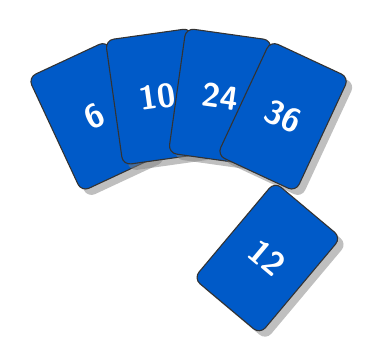
\begin{tikzpicture}[
					% Định nghĩa style cho lá bài
					card/.style={
						draw=black!80, 
						fill=codeblue, % Dùng màu codeblue từ file week8.tex
						text=white,
						minimum width=1.1cm, 
						minimum height=1.6cm,
						rounded corners=3pt, 
						font=\sffamily\bfseries\large,
						anchor=center,
						drop shadow % Tạo bóng nhẹ cho giống thật (cần \usetikzlibrary{shadows})
					}
					]
					% Vẽ các lá bài đang xòe trên tay (Fan shape)
					% Tinh chỉnh toạ độ và góc xoay (rotate) để giống hình
					\node[card, rotate=25]  at (0, 0)      {6};
					\node[card, rotate=8]   at (0.8, 0.25) {10};
					\node[card, rotate=-8]  at (1.6, 0.25) {24};
					\node[card, rotate=-25] at (2.4, 0)    {36};
					
					% Lá bài số 12 nằm riêng phía dưới
					\node[card, rotate=-40] at (2.2, -1.8) {12};
				\end{tikzpicture}
			\end{column}
			
			% --- CỘT PHẢI: Văn bản giải thích ---
			\begin{column}{0.55\textwidth}
				\vspace{0.8cm} % Căn chỉnh cho ngang tầm với bộ bài
				\large
				\bfseries
				\color{HUSTRed}
				Để chèn 12, ta cần tạo chỗ cho nó bởi việc dịch chuyển đầu tiên là 36 và sau đó là 24.
			\end{column}
		\end{columns}
	\end{frame}
	
	% ==================================================================
	% SLIDE 17: Bước 1 - Dịch chuyển lá 36
	% ==================================================================
	\begin{frame}[t]{2. SẮP XẾP CHÈN}
		\setlength{\leftmargini}{-1.2em}
		
		% --- Khung văn bản (Trong suốt) ---
		\begin{tcolorbox}[
			standard jigsaw, opacityback=0,
			colframe=codeblue!50, boxrule=0.5pt, arc=0pt,
			left=6pt, right=6pt, top=6pt, bottom=6pt
			]
			\color{green!60!black}
			\large
			Phỏng theo cách làm của người chơi bài khi cần "chèn" thêm một con bài vào bộ bài đã được sắp xếp trên tay.
		\end{tcolorbox}
		
		\vspace{0.5cm}
		
		\begin{columns}[T, onlytextwidth]
			% --- CỘT TRÁI: Hình vẽ ---
			\begin{column}{0.45\textwidth}
				\centering
				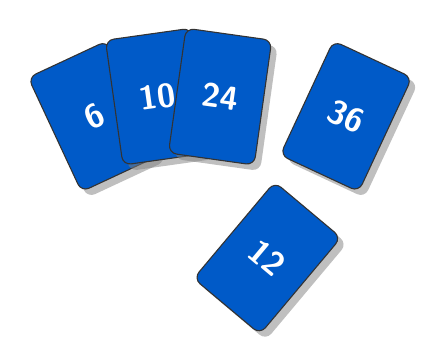
\begin{tikzpicture}[
					card/.style={
						draw=black!80, fill=codeblue, text=white,
						minimum width=1.1cm, minimum height=1.6cm,
						rounded corners=3pt, font=\sffamily\bfseries\large,
						anchor=center, drop shadow
					}
					]
					% 6, 10, 24 giữ nguyên vị trí
					\node[card, rotate=25]  at (0, 0)      {6};
					\node[card, rotate=8]   at (0.8, 0.25) {10};
					\node[card, rotate=-8]  at (1.6, 0.25) {24};
					
					% 36 bị đẩy sang phải để tạo chỗ (Dịch x từ 2.4 -> 3.2)
					\node[card, rotate=-25] at (3.2, 0)    {36};
					
					% 12 vẫn nằm chờ bên dưới
					\node[card, rotate=-40] at (2.2, -1.8) {12};
				\end{tikzpicture}
			\end{column}
			
			% --- CỘT PHẢI: Văn bản ---
			\begin{column}{0.55\textwidth}
				\vspace{0.8cm}
				\large \bfseries \color{red!80!black}
				Để chèn 12, ta cần tạo chỗ cho nó bởi việc dịch chuyển đầu tiên là 36 và sau đó là 24.
			\end{column}
		\end{columns}
	\end{frame}
	
	% ==================================================================
	% SLIDE 18: Bước 2 - Dịch chuyển lá 24
	% ==================================================================
	\begin{frame}[t]{2. SẮP XẾP CHÈN}
		\setlength{\leftmargini}{-1.2em}
		
		\begin{tcolorbox}[
			standard jigsaw, opacityback=0,
			colframe=codeblue!50, boxrule=0.5pt, arc=0pt,
			left=6pt, right=6pt, top=6pt, bottom=6pt
			]
			\color{green!60!black}
			\large
			Phỏng theo cách làm của người chơi bài khi cần "chèn" thêm một con bài vào bộ bài đã được sắp xếp trên tay.
		\end{tcolorbox}
		
		\vspace{0.5cm}
		
		\begin{columns}[T, onlytextwidth]
			\begin{column}{0.45\textwidth}
				\centering
				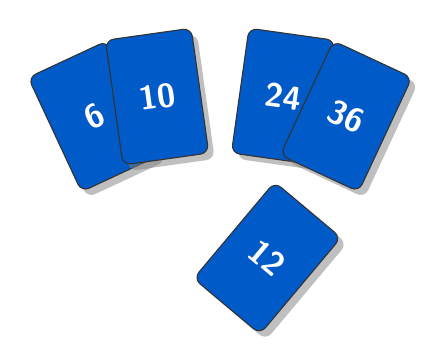
\begin{tikzpicture}[
					card/.style={
						draw=black!80, fill=codeblue, text=white,
						minimum width=1.1cm, minimum height=1.6cm,
						rounded corners=3pt, font=\sffamily\bfseries\large,
						anchor=center, drop shadow
					}
					]
					% 6, 10 giữ nguyên
					\node[card, rotate=25]  at (0, 0)      {6};
					\node[card, rotate=8]   at (0.8, 0.25) {10};
					
					% 24 bị đẩy sang phải (Dịch x từ 1.6 -> 2.4)
					\node[card, rotate=-8]  at (2.4, 0.25) {24};
					
					% 36 giữ nguyên vị trí đã dịch ở slide trước
					\node[card, rotate=-25] at (3.2, 0)    {36};
					
					% 12 vẫn nằm chờ bên dưới
					\node[card, rotate=-40] at (2.2, -1.8) {12};
				\end{tikzpicture}
			\end{column}
			
			\begin{column}{0.55\textwidth}
				\vspace{0.8cm}
				\large \bfseries \color{red!80!black}
				Để chèn 12, ta cần tạo chỗ cho nó bởi việc dịch chuyển đầu tiên là 36 và sau đó là 24.
			\end{column}
		\end{columns}
	\end{frame}
	
	% ==================================================================
	% SLIDE 19: Hoàn tất - Chèn 12 vào vị trí
	% ==================================================================
	\begin{frame}[t]{2. SẮP XẾP CHÈN}
		\setlength{\leftmargini}{-1.2em}
		
		\begin{tcolorbox}[
			standard jigsaw, opacityback=0,
			colframe=codeblue!50, boxrule=0.5pt, arc=0pt,
			left=6pt, right=6pt, top=6pt, bottom=6pt
			]
			\color{green!60!black}
			\large
			Phỏng theo cách làm của người chơi bài khi cần "chèn" thêm một con bài vào bộ bài đã được sắp xếp trên tay.
		\end{tcolorbox}
		
		\vspace{0.5cm}
		
		\begin{columns}[T, onlytextwidth]
			\begin{column}{0.45\textwidth}
				\centering
				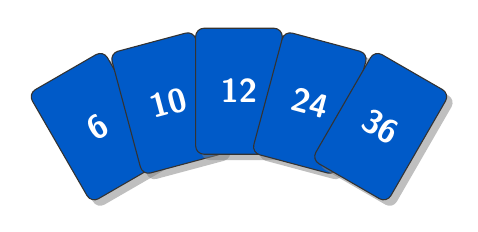
\begin{tikzpicture}[
					card/.style={
						draw=black!80, fill=codeblue, text=white,
						minimum width=1.1cm, minimum height=1.6cm,
						rounded corners=3pt, font=\sffamily\bfseries\large,
						anchor=center, drop shadow
					}
					]
					% Vẽ lại toàn bộ 5 lá bài thành hình quạt cân đối
					% Tinh chỉnh tọa độ và góc xoay để giống ảnh cuối
					\node[card, rotate=30]  at (0, 0)      {6};
					\node[card, rotate=15]  at (0.9, 0.3)  {10};
					\node[card, rotate=0]   at (1.8, 0.45) {12}; % Lá 12 chèn vào giữa
					\node[card, rotate=-15] at (2.7, 0.3)  {24};
					\node[card, rotate=-30] at (3.6, 0)    {36};
				\end{tikzpicture}
			\end{column}
			
			\begin{column}{0.55\textwidth}
				\vspace{0.8cm}
				\large \bfseries \color{red!80!black}
				Để chèn 12, ta cần tạo chỗ cho nó bởi việc dịch chuyển đầu tiên là 36 và sau đó là 24.
			\end{column}
		\end{columns}
	\end{frame}
	
	\begin{frame}[t,fragile]{2. SẮP XẾP CHÈN}
		\small
		
		\vspace{-0.35cm}
		\begin{tcolorbox}[
			width=\textwidth,
			colback=white,
			colframe=blue!60,
			boxrule=0.8pt,
			arc=0pt,
			left=6pt,right=6pt,top=4pt,bottom=4pt
			]
			\textbf{Thuật toán:}
			\begin{itemize}
				\item Tại bước \textcolor{red}{$k=1,\,2,\,\ldots,\,n$}, đưa phần tử thứ $k$ trong mảng đã cho vào đúng vị trí trong dãy gồm $k$ phần tử đầu tiên.
				\item Kết quả là sau bước \textcolor{red}{$k$}, $k$ phần tử đầu tiên là được sắp thứ tự.
			\end{itemize}
		\end{tcolorbox}
		
		\vspace{-0.65cm}
		
		% --- 2 khối dưới: Giải thích (trái) + Code (phải) ---
		\begin{columns}[T,totalwidth=\textwidth]
			\begin{column}{0.42\textwidth}
				\begin{tcolorbox}[
					width=\linewidth,
					colback=white,
					colframe=blue!60,
					boxrule=0.8pt,
					arc=0pt,
					left=0pt,right=6pt,top=0pt,bottom=6pt
					]
					{\color{black}\textbf{Giải thích:}}
					
					{\small\color{yellow}
						\begin{itemize}
							\item Ở đầu lần lặp $i$ của vòng \texttt{"for"} ngoài, dữ liệu từ \texttt{a[0]} đến \texttt{a[i-1]} là được sắp xếp.
							\item Vòng lặp \texttt{"while"} tìm vị trí cho phần tử tiếp theo \texttt{(last = a[i])} trong dãy gồm $i$ phần tử đầu tiên.
						\end{itemize}
					}
					
				\end{tcolorbox}
			\end{column}
			
			
			% ---- Right: Code ----
			\begin{column}{0.58\textwidth}
				\begin{tcolorbox}[
					width=\linewidth,
					colback=white,
					colframe=blue!60,
					boxrule=0.8pt,
					arc=0pt,
					left=-30pt,right=6pt,top=0pt,bottom=6pt
					]
					\begin{minted}[
						fontsize=\scriptsize,
						breaklines,
						linenos=false
						]{c}
						void insertionSort(int a[], int array_size) {
							int i, j, last;
							for (i = 1; i < array_size; i++) {
								last = a[i];
								j = i;
								while ((j > 0) && (a[j-1] > last)) {
									a[j] = a[j-1];
									j = j - 1; } // end while
								a[j] = last;
							} // end for
						} // end of isort
					\end{minted}
				\end{tcolorbox}
			\end{column}
		\end{columns}
		
	\end{frame}
	
	% ==================================================================
	% SLIDE 21: VÍ DỤ MINH HỌA (Đã sửa mũi tên 2 chiều)
	% ==================================================================
	\begin{frame}[t]{2. SẮP XẾP CHÈN}
		\textbf{\large $\gg$ \ Ví dụ}
		
		\vspace{-0.75cm}
		\begin{center}
			\begin{adjustbox}{width=0.60\textwidth}
				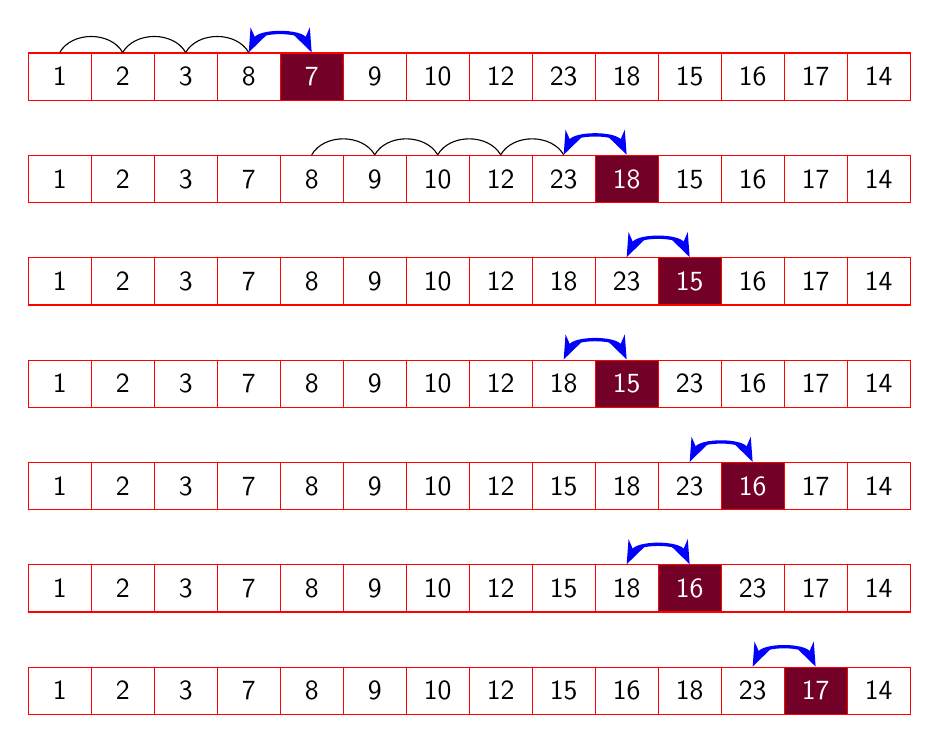
\begin{tikzpicture}[
					x=0.8cm, y=1.3cm, % Tăng khoảng cách y để mũi tên không bị dính
					cell/.style={
						draw=red,             % Viền đỏ
						minimum width=0.8cm, 
						minimum height=0.6cm,
						font=\sffamily,
						anchor=center
					},
					hl/.style={               % Ô được chọn (màu tím đậm)
						fill=purple!60!black,
						text=white
					},
					% --- SỬA LẠI: Mũi tên xanh 2 chiều (<->), cong lên trên ---
					arrow_swap/.style={
						<->, >=Stealth, 
						blue, line width=1.2pt,
						bend right=65         % Độ cong
					},
					arrow_scan/.style={       % Mũi tên đen (duyệt)
						-, 
						black, thin,
						bend left=60
					}
					]
					% --- HÀNG 1 ---
					% Data: 1 2 3 8 [7] 9 10 12 23 18 15 16 17 14
					\foreach \val [count=\i] in {1, 2, 3, 8, 7, 9, 10, 12, 23, 18, 15, 16, 17, 14} {
						\ifnum\i=5
						\node[cell, hl] (r1-\i) at (\i, 0) {\val};
						\else
						\node[cell] (r1-\i) at (\i, 0) {\val};
						\fi
					}
					% Mũi tên đen nối các phần tử đã sắp xếp
					\foreach \x [evaluate=\x as \nextx using int(\x+1)] in {1, 2, 3} {
						\draw[arrow_scan] (r1-\x.north) to (r1-\nextx.north);
					}
					% Mũi tên xanh 2 chiều: so sánh 8 và 7
					\draw[arrow_swap] (r1-5.north) to (r1-4.north);
					
					% --- HÀNG 2 ---
					% Data: 1 2 3 7 8 9 10 12 23 [18] 15 16 17 14
					\foreach \val [count=\i] in {1, 2, 3, 7, 8, 9, 10, 12, 23, 18, 15, 16, 17, 14} {
						\ifnum\i=10
						\node[cell, hl] (r2-\i) at (\i, -1) {\val};
						\else
						\node[cell] (r2-\i) at (\i, -1) {\val};
						\fi
					}
					% Mũi tên đen
					\foreach \x [evaluate=\x as \nextx using int(\x+1)] in {5, ..., 8} {
						\draw[arrow_scan] (r2-\x.north) to (r2-\nextx.north);
					}
					% Mũi tên xanh 2 chiều: so sánh 23 và 18
					\draw[arrow_swap] (r2-10.north) to (r2-9.north);
					
					% --- HÀNG 3 ---
					% Data: ... 12 18 23 [15] ...
					\foreach \val [count=\i] in {1, 2, 3, 7, 8, 9, 10, 12, 18, 23, 15, 16, 17, 14} {
						\ifnum\i=11
						\node[cell, hl] (r3-\i) at (\i, -2) {\val};
						\else
						\node[cell] (r3-\i) at (\i, -2) {\val};
						\fi
					}
					% Mũi tên xanh 2 chiều: so sánh 23 và 15
					\draw[arrow_swap] (r3-11.north) to (r3-10.north);
					
					% --- HÀNG 4 ---
					% Data: ... 12 18 [15] 23 ...
					\foreach \val [count=\i] in {1, 2, 3, 7, 8, 9, 10, 12, 18, 15, 23, 16, 17, 14} {
						\ifnum\i=10
						\node[cell, hl] (r4-\i) at (\i, -3) {\val};
						\else
						\node[cell] (r4-\i) at (\i, -3) {\val};
						\fi
					}
					% Mũi tên xanh 2 chiều: so sánh 18 và 15
					\draw[arrow_swap] (r4-10.north) to (r4-9.north);
					
					% --- HÀNG 5 ---
					% Data: ... 15 18 23 [16] ...
					\foreach \val [count=\i] in {1, 2, 3, 7, 8, 9, 10, 12, 15, 18, 23, 16, 17, 14} {
						\ifnum\i=12
						\node[cell, hl] (r5-\i) at (\i, -4) {\val};
						\else
						\node[cell] (r5-\i) at (\i, -4) {\val};
						\fi
					}
					% Mũi tên xanh 2 chiều: so sánh 23 và 16
					\draw[arrow_swap] (r5-12.north) to (r5-11.north);
					
					% --- HÀNG 6 ---
					% Data: ... 15 18 [16] 23 ...
					\foreach \val [count=\i] in {1, 2, 3, 7, 8, 9, 10, 12, 15, 18, 16, 23, 17, 14} {
						\ifnum\i=11
						\node[cell, hl] (r6-\i) at (\i, -5) {\val};
						\else
						\node[cell] (r6-\i) at (\i, -5) {\val};
						\fi
					}
					% Mũi tên xanh 2 chiều: so sánh 18 và 16
					\draw[arrow_swap] (r6-11.north) to (r6-10.north);
					
					% --- HÀNG 7 ---
					% Data: ... 16 18 23 [17] ...
					\foreach \val [count=\i] in {1, 2, 3, 7, 8, 9, 10, 12, 15, 16, 18, 23, 17, 14} {
						\ifnum\i=13
						\node[cell, hl] (r7-\i) at (\i, -6) {\val};
						\else
						\node[cell] (r7-\i) at (\i, -6) {\val};
						\fi
					}
					% Mũi tên xanh 2 chiều: so sánh 23 và 17
					\draw[arrow_swap] (r7-13.north) to (r7-12.north);
					
				\end{tikzpicture}
			\end{adjustbox}
		\end{center}
	\end{frame}
	
	% ==================================================================
	% SLIDE 22: VÍ DỤ MINH HỌA (TIẾP THEO)
	% ==================================================================
	\begin{frame}[t]{2. SẮP XẾP CHÈN}
		\textbf{\large \ \ $\gg$ \ Ví dụ}
		
		\begin{columns}[T, onlytextwidth]
			% --- CỘT TRÁI: Thống kê ---
			\begin{column}{0.30\textwidth}
				\large
				% Đổi từ bend right -> bend left để mũi tên vồng lên trên
				13 phép đổi chỗ: \ \tikz[baseline=-5pt] \draw[blue, line width=1.2pt, <->, >=Stealth, bend left=60] (0,0) to (0.8,0);
				
				\vspace{0.6cm}
				% Vẽ icon cung tròn đen
				20 phép so sánh: \ \tikz[baseline=-5pt] \draw[black, thin, -, bend left=60] (0,0) to (0.8,0);
			\end{column}
			
			% --- CỘT PHẢI: Hình vẽ các bước cuối ---
			\begin{column}{0.60\textwidth}
				\vspace{-0.75cm}
				\begin{adjustbox}{width=1\textwidth}
					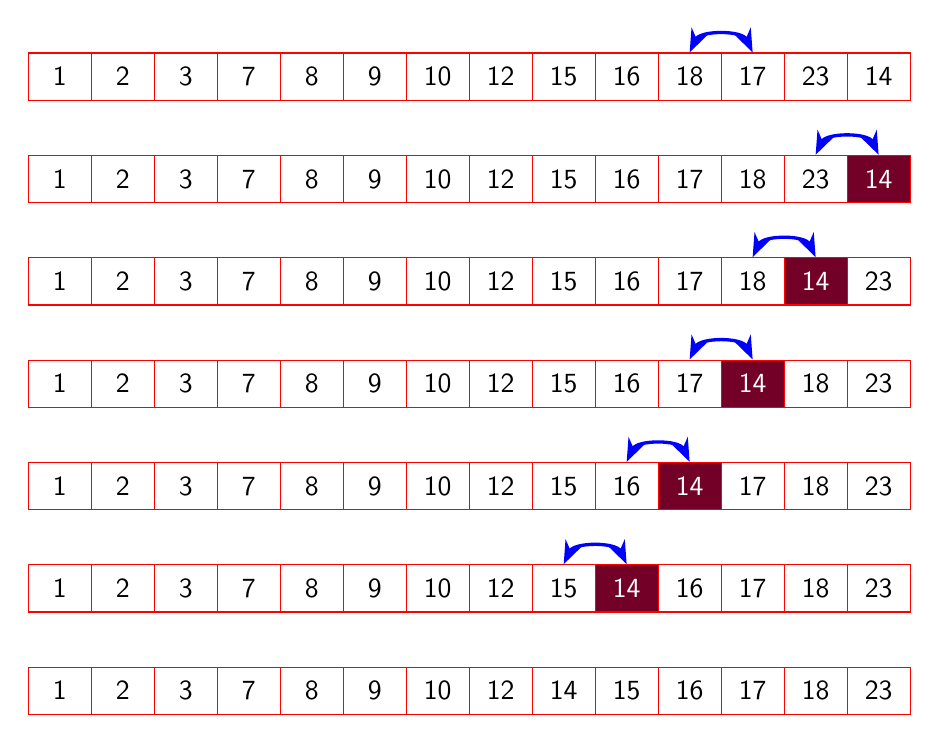
\begin{tikzpicture}[
						x=0.8cm, y=1.3cm, 
						cell/.style={
							draw=red,             % Viền đỏ
							minimum width=0.8cm, 
							minimum height=0.6cm,
							font=\sffamily,
							anchor=center
						},
						hl/.style={               % Ô được chọn (màu tím đậm)
							fill=purple!60!black,
							text=white
						},
						arrow_swap/.style={       % Mũi tên xanh 2 chiều
							<->, >=Stealth, 
							blue, line width=1.2pt,
							bend right=65
						}
						]
						% --- HÀNG 1: Đổi chỗ 17 và 18 (tiếp nối slide trước) ---
						% Data: 1 2 3 7 8 9 10 12 15 16 [18] [17] 23 14
						\foreach \val [count=\i] in {1, 2, 3, 7, 8, 9, 10, 12, 15, 16, 18, 17, 23, 14} {
							\node[cell] (r1-\i) at (\i, 0) {\val};
						}
						% Swap 18 (vt 11) và 17 (vt 12)
						\draw[arrow_swap] (r1-12.north) to (r1-11.north); 
						
						% --- HÀNG 2: Bắt đầu chèn 14 ---
						% Data: ... 17 18 23 [14]
						\foreach \val [count=\i] in {1, 2, 3, 7, 8, 9, 10, 12, 15, 16, 17, 18, 23, 14} {
							\ifnum\i=14 
							\node[cell, hl] (r2-\i) at (\i, -1) {\val}; 
							\else 
							\node[cell] (r2-\i) at (\i, -1) {\val}; 
							\fi
						}
						% Swap 14 (vt 14) và 23 (vt 13)
						\draw[arrow_swap] (r2-14.north) to (r2-13.north);
						
						% --- HÀNG 3 ---
						% Data: ... 17 18 [14] 23
						\foreach \val [count=\i] in {1, 2, 3, 7, 8, 9, 10, 12, 15, 16, 17, 18, 14, 23} {
							\ifnum\i=13 
							\node[cell, hl] (r3-\i) at (\i, -2) {\val}; 
							\else 
							\node[cell] (r3-\i) at (\i, -2) {\val}; 
							\fi
						}
						% Swap 14 (vt 13) và 18 (vt 12)
						\draw[arrow_swap] (r3-13.north) to (r3-12.north);
						
						% --- HÀNG 4 ---
						% Data: ... 17 [14] 18 23
						\foreach \val [count=\i] in {1, 2, 3, 7, 8, 9, 10, 12, 15, 16, 17, 14, 18, 23} {
							\ifnum\i=12 
							\node[cell, hl] (r4-\i) at (\i, -3) {\val}; 
							\else 
							\node[cell] (r4-\i) at (\i, -3) {\val}; 
							\fi
						}
						% Swap 14 (vt 12) và 17 (vt 11)
						\draw[arrow_swap] (r4-12.north) to (r4-11.north);
						
						% --- HÀNG 5 ---
						% Data: ... 16 [14] 17 18 23
						\foreach \val [count=\i] in {1, 2, 3, 7, 8, 9, 10, 12, 15, 16, 14, 17, 18, 23} {
							\ifnum\i=11 
							\node[cell, hl] (r5-\i) at (\i, -4) {\val}; 
							\else 
							\node[cell] (r5-\i) at (\i, -4) {\val}; 
							\fi
						}
						% Swap 14 (vt 11) và 16 (vt 10)
						\draw[arrow_swap] (r5-11.north) to (r5-10.north);
						
						% --- HÀNG 6 ---
						% Data: ... 15 [14] 16 17 18 23
						\foreach \val [count=\i] in {1, 2, 3, 7, 8, 9, 10, 12, 15, 14, 16, 17, 18, 23} {
							\ifnum\i=10 
							\node[cell, hl] (r6-\i) at (\i, -5) {\val}; 
							\else 
							\node[cell] (r6-\i) at (\i, -5) {\val}; 
							\fi
						}
						% Swap 14 (vt 10) và 15 (vt 9)
						\draw[arrow_swap] (r6-10.north) to (r6-9.north);
						
						% --- HÀNG 7 (Hoàn tất) ---
						% Data: ... 14 15 16 17 18 23
						\foreach \val [count=\i] in {1, 2, 3, 7, 8, 9, 10, 12, 14, 15, 16, 17, 18, 23} {
							\node[cell] (r7-\i) at (\i, -6) {\val};
						}
						
					\end{tikzpicture}
				\end{adjustbox}
			\end{column}
		\end{columns}
	\end{frame}
	
	\begin{frame}[t]{2. SẮP XẾP CHÈN}
		\setlength{\leftmargini}{-1.2em}
		\small
		
		\begin{itemize}
			\item Các đặc tính của sắp xếp chèn
			
			\vspace{0.25cm}
			
			\item \textbf{Tại chỗ và ổn định (In place and Stable)}
			
			\vspace{0.25cm}
			
			\item \textbf{Thời gian tính}
			\begin{itemize}
				\item \textbf{\textit{Best Case:}} $0$ hoán đổi, $n-1$ so sánh \textit{(khi dãy đầu vào là đã được sắp)}
				\item \textbf{\textit{Worst Case:}} $n^2/2$ hoán đổi và so sánh \textit{(khi dãy đầu vào có thứ tự ngược lại với thứ tự cần sắp xếp)}
			\end{itemize}
			
			\vspace{0.15cm}
			
			\item Thuật toán sắp xếp tốt đối với dãy đã gần được sắp xếp
			\begin{itemize}
				\item Mỗi phần tử đã đứng ở vị trí rất gần vị trí trong thứ tự cần sắp xếp
			\end{itemize}
		\end{itemize}
		
	\end{frame}
	
	% ==================================================================
	% SLIDE 27: SẮP XẾP CHỌN - VÍ DỤ
	% ==================================================================
	\begin{frame}[t]{3. SẮP XẾP CHỌN}
		\vspace{0.2cm}
		\textbf{\large $\gg$ \ Ví dụ}
		
		\vspace{-0.75cm}
		\begin{center}
			\begin{adjustbox}{width=0.6\textwidth}
			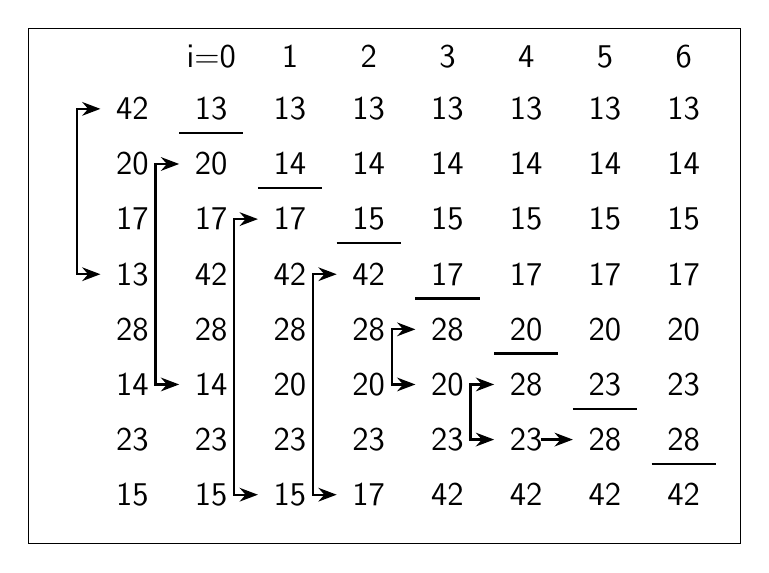
\begin{tikzpicture}[
				font=\sffamily\large,
				% Style cho các ô số
				mynode/.style={minimum width=0.8cm, minimum height=0.6cm, anchor=center},
				% Style cho mũi tên hoán đổi (đen, 2 đầu)
				swap_arrow/.style={
					<->, >=Stealth, 
					black, line width=0.8pt
				}
				]
				% --- BẢNG DỮ LIỆU (MATRIX) ---
				\matrix (m) [
				matrix of nodes,
				nodes={mynode},
				column sep=0.2cm,
				row sep=0.1cm,
				ampersand replacement=\&
				] {
					% Row 1
					42 \& 13 \& 13 \& 13 \& 13 \& 13 \& 13 \& 13 \\
					% Row 2
					20 \& 20 \& 14 \& 14 \& 14 \& 14 \& 14 \& 14 \\
					% Row 3
					17 \& 17 \& 17 \& 15 \& 15 \& 15 \& 15 \& 15 \\
					% Row 4
					13 \& 42 \& 42 \& 42 \& 17 \& 17 \& 17 \& 17 \\
					% Row 5
					28 \& 28 \& 28 \& 28 \& 28 \& 20 \& 20 \& 20 \\
					% Row 6
					14 \& 14 \& 20 \& 20 \& 20 \& 28 \& 23 \& 23 \\
					% Row 7
					23 \& 23 \& 23 \& 23 \& 23 \& 23 \& 28 \& 28 \\
					% Row 8
					15 \& 15 \& 15 \& 17 \& 42 \& 42 \& 42 \& 42 \\
				};
				
				% --- TIÊU ĐỀ CỘT (i=0, 1, 2...) ---
				\node[above=0.1cm of m-1-2] {i=0};
				\node[above=0.1cm of m-1-3] {1};
				\node[above=0.1cm of m-1-4] {2};
				\node[above=0.1cm of m-1-5] {3};
				\node[above=0.1cm of m-1-6] {4};
				\node[above=0.1cm of m-1-7] {5};
				\node[above=0.1cm of m-1-8] {6};
				
				% --- GẠCH CHÂN CÁC SỐ ĐÃ SẮP XẾP ---
				% i=0: gạch chân 13
				\draw[black, thick] (m-1-2.south west) -- (m-1-2.south east);
				% i=1: gạch chân 14
				\draw[black, thick] (m-2-3.south west) -- (m-2-3.south east);
				% i=2: gạch chân 15
				\draw[black, thick] (m-3-4.south west) -- (m-3-4.south east);
				% i=3: gạch chân 17
				\draw[black, thick] (m-4-5.south west) -- (m-4-5.south east);
				% i=4: gạch chân 20
				\draw[black, thick] (m-5-6.south west) -- (m-5-6.south east);
				% i=5: gạch chân 23
				\draw[black, thick] (m-6-7.south west) -- (m-6-7.south east);
				% i=6: gạch chân 28 và 42
				\draw[black, thick] (m-7-8.south west) -- (m-7-8.south east);
				
				
				% --- VẼ CÁC MŨI TÊN HOÁN ĐỔI ---
				
				% Cột 1 (Ban đầu): Swap 42 (r1) <-> 13 (r4)
				\draw[swap_arrow] (m-1-1.west) -- ++(-0.3,0) |- (m-4-1.west);
				
				% Cột 2 (i=0): Swap 20 (r2) <-> 14 (r6)
				\draw[swap_arrow] (m-2-2.west) -- ++(-0.3,0) |- (m-6-2.west);
				
				% Cột 3 (i=1): Swap 17 (r3) <-> 15 (r8)
				\draw[swap_arrow] (m-3-3.west) -- ++(-0.3,0) |- (m-8-3.west);
				
				% Cột 4 (i=2): Swap 42 (r4) <-> 17 (r8)
				\draw[swap_arrow] (m-4-4.west) -- ++(-0.3,0) |- (m-8-4.west);
				
				% Cột 5 (i=3): Swap 28 (r5) <-> 20 (r6)
				\draw[swap_arrow] (m-5-5.west) -- ++(-0.3,0) |- (m-6-5.west);
				
				% Cột 6 (i=4): Swap 28 (r6) <-> 23 (r7)
				\draw[swap_arrow] (m-6-6.west) -- ++(-0.3,0) |- (m-7-6.west);
				
				% Cột 7 (i=5): Swap 28 (r7) <-> 28 (r7) (Chính nó)
				% Vẽ mũi tên nhỏ chỉ vào chính nó
				\draw[<-, >=Stealth, black, line width=0.8pt] (m-7-7.west) -- ++(-0.4,0);
				
				% --- KHUNG BAO NGOÀI ---
				\draw[black, thin] ($(m.north west)+(-0.8,0.6)$) rectangle ($(m.south east)+(0.2,-0.2)$);
				
			\end{tikzpicture}
			\end{adjustbox}
		\end{center}
	\end{frame}
	
	\subsection{Sắp xếp chọn}
	
	% =========================
	% SLIDE 25: 3. SẮP XẾP CHỌN (Thuật toán + code)
	% =========================
	\begin{frame}[t,fragile]{3. SẮP XẾP CHỌN}
		\setlength{\leftmargini}{-1.2em}
		\small
		
		\vspace{-0.25cm}
		
		\begin{columns}[T,totalwidth=\textwidth]
			% ---- Left: thuật toán ----
			\begin{column}{0.54\textwidth}
				\begin{itemize}
					\item[$\triangleright$] Thuật toán
					
					\vspace{0.15cm}
					\item Tìm phần tử nhỏ nhất đưa vào vị trí 1
					\item Tìm phần tử nhỏ tiếp theo đưa vào vị trí 2
					\item Tìm phần tử nhỏ tiếp theo đưa vào vị trí 3
				\end{itemize}
				
				\hspace{1.05em}\ldots
			\end{column}
			
			% ---- Right: code boxes ----
			\begin{column}{0.46\textwidth}
				% swap box (nhỏ, canh phải)
				\hfill
				\begin{tcolorbox}[
					width=0.65\linewidth,
					colback=blue!4,
					colframe=blue!60,
					boxrule=0.8pt,
					arc=0pt,
					left=-40pt,right=6pt,top=6pt,bottom=6pt
					]
					\begin{minted}[fontsize=\scriptsize,breaklines,linenos=false]{cpp}
						void swap(int &a,int &b){
							int temp = a;
							a = b;
							b = temp;
						}
					\end{minted}
				\end{tcolorbox}
				
				% selectionSort box (lớn)
				\begin{tcolorbox}[
					width=\linewidth,
					colback=blue!4,
					colframe=blue!60,
					boxrule=0.8pt,
					arc=0pt,
					left=-40pt,right=6pt,top=0pt,bottom=6pt
					]
					\begin{minted}[fontsize=\scriptsize,breaklines,linenos=false]{cpp}
						void selectionSort(int a[], int n){
							int i, j, min, temp;
							for (i = 0; i < n-1; i++) {
								min = i;
								for (j = i+1; j < n; j++){
									if (a[j] < a[min]) min = j;
								}
								swap(a[i], a[min]);
							}
						}
					\end{minted}
				\end{tcolorbox}
			\end{column}
		\end{columns}
		
	\end{frame}
	
	% =========================
	% SLIDE 26: 3. SẮP XẾP CHỌN (Nhận xét)
	% =========================
	\begin{frame}[t]{3. SẮP XẾP CHỌN}
		\setlength{\leftmargini}{-1.2em}
		\small
		
		\begin{itemize}
			\item[$\triangleright$] Nhận xét
			
			\vspace{0.15cm}
			
			\item \textbf{Best case:} $0$ đổi chỗ \textit{(n-1 như trong đoạn mã)}, $n^2/2$ so sánh.
			\item \textbf{Worst case:} $n-1$ đổi chỗ và $n^2/2$ so sánh.
			\item \textbf{Average case:} $O(n)$ đổi chỗ và $n^2/2$ so sánh.
			
			\vspace{0.1cm}
			
			\item \textcolor{blue}{\textbf{Ưu điểm nổi bật:} số phép đổi chỗ ít.}
			\begin{itemize}
				\item Có ý nghĩa nếu như thao tác đổi chỗ tốn kém.
			\end{itemize}
		\end{itemize}
		
	\end{frame}
	
	% ==================================================================
	% SLIDE 27: SẮP XẾP CHỌN - VÍ DỤ (ĐÃ THU NHỎ)
	% ==================================================================
	\begin{frame}[t]{3. SẮP XẾP CHỌN}
		
		\textbf{\large $\gg$ \ Ví dụ}
		\vspace*{-0.3cm}
		\begin{center}

			\begin{adjustbox}{max width=1\textwidth}
				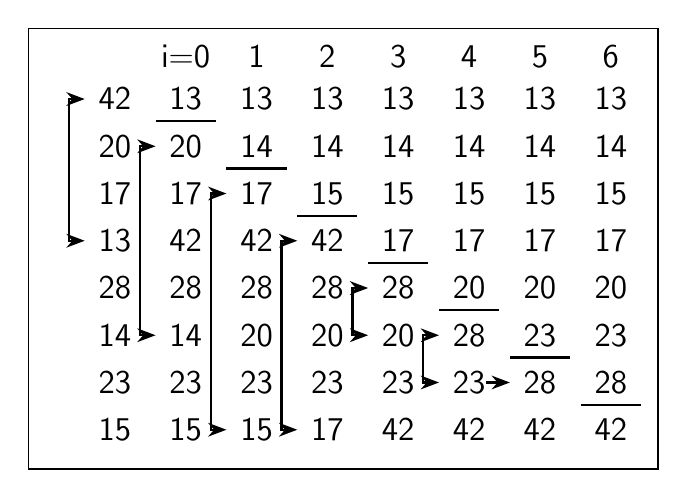
\begin{tikzpicture}[
					font=\sffamily\large,
					% Giảm kích thước ô một chút cho gọn
					mynode/.style={minimum width=0.75cm, minimum height=0.55cm, anchor=center},
					swap_arrow/.style={
						<->, >=Stealth, 
						black, line width=0.8pt
					}
					]
					% --- BẢNG DỮ LIỆU (MATRIX) ---
					\matrix (m) [
					matrix of nodes,
					nodes={mynode},
					column sep=0.15cm, % Giảm khoảng cách cột
					row sep=0.05cm,    % Giảm khoảng cách hàng
					ampersand replacement=\&
					] {
						% Row 1
						42 \& 13 \& 13 \& 13 \& 13 \& 13 \& 13 \& 13 \\
						20 \& 20 \& 14 \& 14 \& 14 \& 14 \& 14 \& 14 \\
						17 \& 17 \& 17 \& 15 \& 15 \& 15 \& 15 \& 15 \\
						13 \& 42 \& 42 \& 42 \& 17 \& 17 \& 17 \& 17 \\
						28 \& 28 \& 28 \& 28 \& 28 \& 20 \& 20 \& 20 \\
						14 \& 14 \& 20 \& 20 \& 20 \& 28 \& 23 \& 23 \\
						23 \& 23 \& 23 \& 23 \& 23 \& 23 \& 28 \& 28 \\
						15 \& 15 \& 15 \& 17 \& 42 \& 42 \& 42 \& 42 \\
					};
					
					% --- TIÊU ĐỀ CỘT ---
					\node[above=0cm of m-1-2] {i=0};
					\node[above=0cm of m-1-3] {1};
					\node[above=0cm of m-1-4] {2};
					\node[above=0cm of m-1-5] {3};
					\node[above=0cm of m-1-6] {4};
					\node[above=0cm of m-1-7] {5};
					\node[above=0cm of m-1-8] {6};
					
					% --- GẠCH CHÂN ---
					\draw[black, thick] (m-1-2.south west) -- (m-1-2.south east);
					\draw[black, thick] (m-2-3.south west) -- (m-2-3.south east);
					\draw[black, thick] (m-3-4.south west) -- (m-3-4.south east);
					\draw[black, thick] (m-4-5.south west) -- (m-4-5.south east);
					\draw[black, thick] (m-5-6.south west) -- (m-5-6.south east);
					\draw[black, thick] (m-6-7.south west) -- (m-6-7.south east);
					\draw[black, thick] (m-7-8.south west) -- (m-7-8.south east);
					
					% --- VẼ CÁC MŨI TÊN HOÁN ĐỔI ---
					% Cột 1: 42 <-> 13
					\draw[swap_arrow] (m-1-1.west) -- ++(-0.2,0) |- (m-4-1.west);
					% Cột 2: 20 <-> 14
					\draw[swap_arrow] (m-2-2.west) -- ++(-0.2,0) |- (m-6-2.west);
					% Cột 3: 17 <-> 15
					\draw[swap_arrow] (m-3-3.west) -- ++(-0.2,0) |- (m-8-3.west);
					% Cột 4: 42 <-> 17
					\draw[swap_arrow] (m-4-4.west) -- ++(-0.2,0) |- (m-8-4.west);
					% Cột 5: 28 <-> 20
					\draw[swap_arrow] (m-5-5.west) -- ++(-0.2,0) |- (m-6-5.west);
					% Cột 6: 28 <-> 23
					\draw[swap_arrow] (m-6-6.west) -- ++(-0.2,0) |- (m-7-6.west);
					% Cột 7: 28 <-> 28 (Mũi tên chỉ vào chính nó)
					\draw[<-, >=Stealth, black, line width=0.8pt] (m-7-7.west) -- ++(-0.3,0);
					
					% --- KHUNG BAO NGOÀI ---
					\draw[black, thin] ($(m.north west)+(-0.6,0.5)$) rectangle ($(m.south east)+(0.1,-0.1)$);
					
				\end{tikzpicture}
			\end{adjustbox}
		\end{center}
	\end{frame}
	
	\subsection{Sắp xếp nổi bọt}
	
	% =========================
	% SLIDE 29: 4. SẮP XẾP NỔI BỌT (Ví dụ)
	% =========================
	\begin{frame}[t]{4. SẮP XẾP NỔI BỌT}
		\setlength{\leftmargini}{-1.2em}
		\small
		
		\begin{itemize}
			\item[$\triangleright$] Ví dụ
			
			\vspace{0.15cm}
			
			\item Bắt đầu từ đầu dãy, thuật toán tiến hành so sánh mỗi phần tử với phần tử đi sau nó và thực hiện đổi chỗ, nếu chúng không theo đúng thứ tự.
			
			\item Quá trình này sẽ được lặp lại cho đến khi gặp lần duyệt từ đầu dãy đến cuối dãy mà không phải thực hiện đổi chỗ (tức là tất cả các phần tử đã đứng đúng vị trí).
			
			\item Cách làm này đã đẩy phần tử lớn nhất xuống cuối dãy, trong khi đó những phần tử có giá trị nhỏ hơn được dịch chuyển về đầu dãy.
		\end{itemize}
		
	\end{frame}
	
	% =========================
	% SLIDE 30: 4. SẮP XẾP NỔI BỌT (Code + Nhận xét)
	% =========================
	\begin{frame}[t,fragile]{4. SẮP XẾP NỔI BỌT}
		\small
		
		\begin{columns}[T,totalwidth=\textwidth]
			% ---- Left: bubbleSort code (to) ----
			\begin{column}{0.45\textwidth}
				\begin{tcolorbox}[
					width=\linewidth,
					colback=blue!4,
					colframe=blue!60,
					boxrule=0.8pt,
					arc=0pt,
					left=-40pt,right=6pt,top=0pt,bottom=6pt
					]
					\begin{minted}[fontsize=\scriptsize,breaklines,linenos=false]{cpp}
						void bubbleSort(int a[], int n){
							int i, j;
							
							for (i = (n-1); i >= 0; i--) {
								for (j = 1; j <= i; j++){
									if (a[j-1] > a[j])
									swap(a[j-1],a[j]);
								}
							}
						}
					\end{minted}
				\end{tcolorbox}
			\end{column}
			
			% ---- Right: swap code + bullets ----
			\begin{column}{0.45\textwidth}
				\begin{tcolorbox}[
					width=\linewidth,
					colback=blue!4,
					colframe=blue!60,
					boxrule=0.8pt,
					arc=0pt,
					left=-30pt,right=6pt,top=0pt,bottom=6pt
					]
					\begin{minted}[fontsize=\scriptsize,breaklines,linenos=false]{cpp}
						void swap(int &a,int &b){
							int temp = a;
							a = b;
							b = temp;
						}
					\end{minted}
				\end{tcolorbox}
				
				\vspace{0.25cm}
				
				\begin{itemize}
					\item Best case: $0$ đổi chỗ, $n^2/2$ so sánh.
					\item Worst case: $n^2/2$ đổi chỗ và so sánh.
					\item Average case: $n^2/4$ đổi chỗ và $n^2/2$ so sánh.
				\end{itemize}
			\end{column}
		\end{columns}
		
	\end{frame}
	
	% ==================================================================
	% SLIDE 31: SẮP XẾP NỔI BỌT
	% ==================================================================
	\begin{frame}[t]{4. SẮP XẾP NỔI BỌT}
		\vspace{-0.35cm}
		
		\begin{center}
			\begin{adjustbox}{width=0.95\textwidth}
				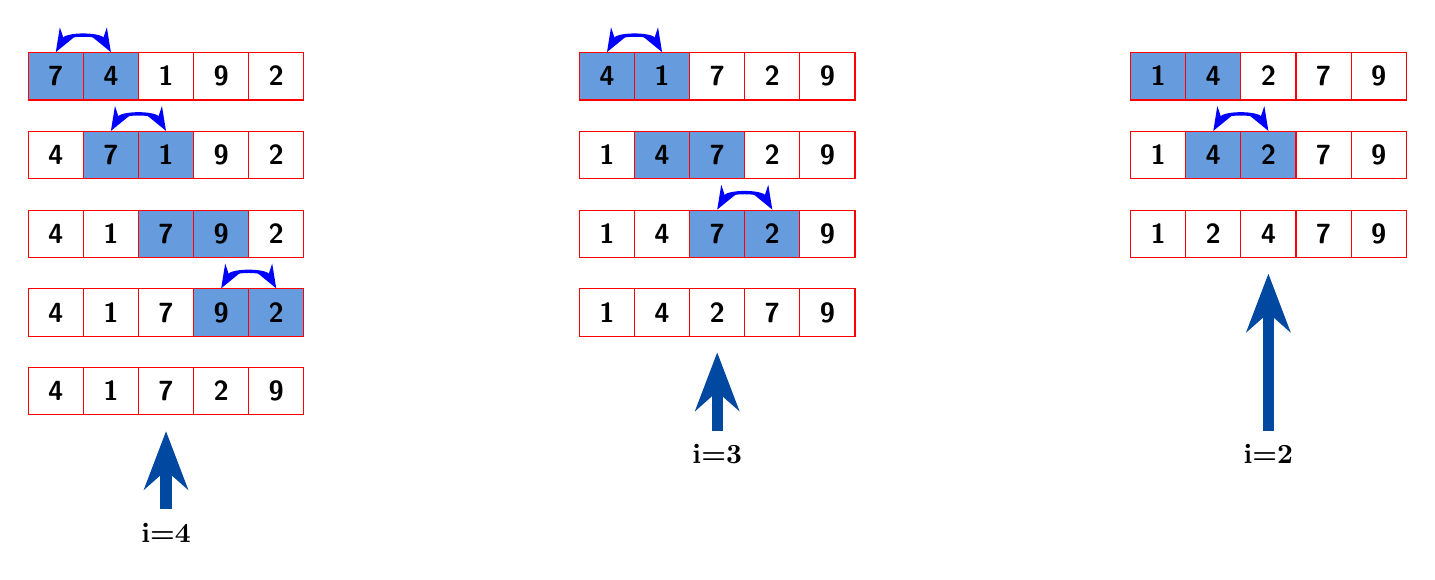
\begin{tikzpicture}[
					x=0.7cm, y=1.0cm,
					cell/.style={
						draw=red, 
						minimum width=0.7cm, 
						minimum height=0.6cm,
						font=\sffamily\bfseries,
						anchor=center
					},
					hi/.style={ % Ô được highlight (đang so sánh)
						fill=codeblue!60, % Màu xanh codeblue nhạt hơn chút
						text=black
					},
					swap_arrow/.style={ % Mũi tên hoán đổi
						<->, >=Stealth, 
						blue, line width=1.2pt,
						bend left=60
					},
					idx_arrow/.style={ % Mũi tên chỉ số i lớn ở dưới
						->, >=Stealth,
						codeblue!80!black,
						line width=4pt,
						shorten >= 3pt
					}
					]
					
					% ================= CỘT 1 (i=4) =================
					% Row 1: 7, 4, 1, 9, 2 (So sánh 7, 4 -> Swap)
					\foreach \val [count=\j] in {7, 4, 1, 9, 2} {
						\ifnum\j<3 \node[cell, hi] (c1r1-\j) at (\j, 0) {\val};
						\else      \node[cell]     (c1r1-\j) at (\j, 0) {\val}; \fi
					}
					\draw[swap_arrow] (c1r1-1.north) to (c1r1-2.north);
					
					% Row 2: 4, 7, 1, 9, 2 (So sánh 7, 1 -> Swap)
					\foreach \val [count=\j] in {4, 7, 1, 9, 2} {
						\ifnum\j>1 \ifnum\j<4 \node[cell, hi] (c1r2-\j) at (\j, -1) {\val};
						\else                 \node[cell]     (c1r2-\j) at (\j, -1) {\val}; \fi
						\else                 \node[cell]     (c1r2-\j) at (\j, -1) {\val}; \fi
					}
					\draw[swap_arrow] (c1r2-2.north) to (c1r2-3.north);
					
					% Row 3: 4, 1, 7, 9, 2 (So sánh 7, 9 -> No Swap)
					\foreach \val [count=\j] in {4, 1, 7, 9, 2} {
						\ifnum\j>2 \ifnum\j<5 \node[cell, hi] (c1r3-\j) at (\j, -2) {\val};
						\else                 \node[cell]     (c1r3-\j) at (\j, -2) {\val}; \fi
						\else                 \node[cell]     (c1r3-\j) at (\j, -2) {\val}; \fi
					}
					% Không vẽ mũi tên swap
					
					% Row 4: 4, 1, 7, 9, 2 (So sánh 9, 2 -> Swap)
					\foreach \val [count=\j] in {4, 1, 7, 9, 2} {
						\ifnum\j>3 \node[cell, hi] (c1r4-\j) at (\j, -3) {\val};
						\else      \node[cell]     (c1r4-\j) at (\j, -3) {\val}; \fi
					}
					\draw[swap_arrow] (c1r4-4.north) to (c1r4-5.north);
					
					% Row 5: 4, 1, 7, 2, 9 (Kết quả bước i=4)
					\foreach \val [count=\j] in {4, 1, 7, 2, 9} {
						\node[cell] (c1r5-\j) at (\j, -4) {\val};
					}
					
					% Mũi tên chỉ số i=4
					\draw[idx_arrow] (3, -5.5) -- (3, -4.4);
					\node[font=\bfseries] at (3, -5.8) {i=4};
					
					
					% ================= CỘT 2 (i=3) =================
					% Shift x = 7
					\begin{scope}[xshift=7cm]
						% Row 1: 4, 1, 7, 2, 9 (So sánh 4, 1 -> Swap)
						\foreach \val [count=\j] in {4, 1, 7, 2, 9} {
							\ifnum\j<3 \node[cell, hi] (c2r1-\j) at (\j, 0) {\val};
							\else      \node[cell]     (c2r1-\j) at (\j, 0) {\val}; \fi
						}
						\draw[swap_arrow] (c2r1-1.north) to (c2r1-2.north);
						
						% Row 2: 1, 4, 7, 2, 9 (So sánh 4, 7 -> No Swap)
						\foreach \val [count=\j] in {1, 4, 7, 2, 9} {
							\ifnum\j>1 \ifnum\j<4 \node[cell, hi] (c2r2-\j) at (\j, -1) {\val};
							\else                 \node[cell]     (c2r2-\j) at (\j, -1) {\val}; \fi
							\else                 \node[cell]     (c2r2-\j) at (\j, -1) {\val}; \fi
						}
						
						% Row 3: 1, 4, 7, 2, 9 (So sánh 7, 2 -> Swap)
						\foreach \val [count=\j] in {1, 4, 7, 2, 9} {
							\ifnum\j>2 \ifnum\j<5 \node[cell, hi] (c2r3-\j) at (\j, -2) {\val};
							\else                 \node[cell]     (c2r3-\j) at (\j, -2) {\val}; \fi
							\else                 \node[cell]     (c2r3-\j) at (\j, -2) {\val}; \fi
						}
						\draw[swap_arrow] (c2r3-3.north) to (c2r3-4.north);
						
						% Row 4: 1, 4, 2, 7, 9 (Kết quả bước i=3)
						\foreach \val [count=\j] in {1, 4, 2, 7, 9} {
							\node[cell] (c2r4-\j) at (\j, -3) {\val};
						}
						
						% Mũi tên chỉ số i=3
						\draw[idx_arrow] (3, -4.5) -- (3, -3.4); % Chỉ vào vị trí index 3 (là số 7)
						\node[font=\bfseries] at (3, -4.8) {i=3};
					\end{scope}
					
					
					% ================= CỘT 3 (i=2) =================
					% Shift x = 14
					\begin{scope}[xshift=14cm]
						% Row 1: 1, 4, 2, 7, 9 (So sánh 1, 4 -> No Swap)
						\foreach \val [count=\j] in {1, 4, 2, 7, 9} {
							\ifnum\j<3 \node[cell, hi] (c3r1-\j) at (\j, 0) {\val};
							\else      \node[cell]     (c3r1-\j) at (\j, 0) {\val}; \fi
						}
						
						% Row 2: 1, 4, 2, 7, 9 (So sánh 4, 2 -> Swap)
						\foreach \val [count=\j] in {1, 4, 2, 7, 9} {
							\ifnum\j>1 \ifnum\j<4 \node[cell, hi] (c3r2-\j) at (\j, -1) {\val};
							\else                 \node[cell]     (c3r2-\j) at (\j, -1) {\val}; \fi
							\else                 \node[cell]     (c3r2-\j) at (\j, -1) {\val}; \fi
						}
						\draw[swap_arrow] (c3r2-2.north) to (c3r2-3.north);
						
						% Row 3: 1, 2, 4, 7, 9 (Kết quả bước i=2)
						\foreach \val [count=\j] in {1, 2, 4, 7, 9} {
							\node[cell] (c3r3-\j) at (\j, -2) {\val};
						}
						
						% Mũi tên chỉ số i=2
						\draw[idx_arrow] (3, -4.5) -- (3, -2.4); % Chỉ vào vị trí index 2 (là số 4)
						\node[font=\bfseries] at (3, -4.8) {i=2};
					\end{scope}
					
				\end{tikzpicture}
			\end{adjustbox}
		\end{center}
		\vspace{-0.35cm}
		\textbf{Chú ý:}
		\begin{itemize}
			\item Các phần tử được đánh chỉ số bắt đầu từ 0.
			\item n=5
		\end{itemize}
	\end{frame}
	
	% ==================================================================
	% SLIDE 32: TỔNG KẾT BA THUẬT TOÁN SẮP XẾP CƠ BẢN
	% ==================================================================
	\begin{frame}[t]{TỔNG KẾT BA THUẬT TOÁN SẮP XẾP CƠ BẢN}
		\begin{center}
			\renewcommand{\arraystretch}{1.5} % Tăng chiều cao dòng cho thoáng
			\setlength{\tabcolsep}{10pt}      % Tăng khoảng cách cột
			
			\begin{adjustbox}{width=0.65\textwidth}
				\begin{tabular}{|l|l|l|l|}
					\hline
					% Hàng tiêu đề
					& \textbf{\textcolor{blue}{Insertion}} & \textbf{\textcolor{blue}{Bubble}} & \textbf{\textcolor{blue}{Selection}} \\
					\cline{2-4}
					
					% --- Phần So sánh ---
					\textbf{\textcolor{red}{Số phép so sánh:}} & & & \\
					\hline
					\textcolor{blue}{Best Case} & \textcolor{blue}{$\Theta(n)$} & \textcolor{blue}{$\Theta(n^2)$} & \textcolor{blue}{$\Theta(n^2)$} \\
					\hline
					\textcolor{blue}{Average Case} & \textcolor{blue}{$\Theta(n^2)$} & \textcolor{blue}{$\Theta(n^2)$} & \textcolor{blue}{$\Theta(n^2)$} \\
					\hline
					\textcolor{blue}{Worst Case} & \textcolor{blue}{$\Theta(n^2)$} & \textcolor{blue}{$\Theta(n^2)$} & \textcolor{blue}{$\Theta(n^2)$} \\
					\hline
					
					% Khoảng trống ngăn cách (tùy chọn)
					\multicolumn{4}{|c|}{} \\[-1.4em] \hline 
					
					% --- Phần Đổi chỗ ---
					\textbf{\textcolor{red}{Số phép đổi chỗ:}} & & & \\
					\hline
					\textcolor{blue}{Best Case} & \textcolor{blue}{$0$} & \textcolor{blue}{$0$} & \textcolor{blue}{$\Theta(n)$} \\
					\hline
					\textcolor{blue}{Average Case} & \textcolor{blue}{$\Theta(n^2)$} & \textcolor{blue}{$\Theta(n^2)$} & \textcolor{blue}{$\Theta(n)$} \\
					\hline
					\textcolor{blue}{Worst Case} & \textcolor{blue}{$\Theta(n^2)$} & \textcolor{blue}{$\Theta(n^2)$} & \textcolor{blue}{$\Theta(n)$} \\
					\hline
				\end{tabular}
			\end{adjustbox}
		\end{center}
	\end{frame}
	
	{\HUSTUseBackground{onelove.pdf}
		\begin{frame}
			\ifdefstring{\insertaspectratio}{169}{
				\HUSTCornerImage[0.14]{assets/logo/soict_vi_h.pdf}
				\placecontent{0.5cm}{0.33\paperheight}{0.85\paperwidth}{
					\color{\HUSTFrameTitleTextColor}\bfseries\fontsize{22pt}{30pt}\selectfont
					\inserttitle
				}
				\placecontent{0.5cm}{0.50\paperheight}{0.8\paperwidth}{
					\color{\HUSTFrameTitleTextColor}\fontsize{14pt}{14pt}\selectfont
					%Bài học
					\textbf{\large TUẦN 10: SẮP XẾP: Sắp xếp trộn (merge sort)}\\
				}
			}{}
		\end{frame}
	}
	
	\section{Merge sort}
	\subsection{Sắp xếp trộn (merge sort)}
	
	\begin{frame}[t]{1. SẮP XẾP TRỘN (MERGE SORT)}
		\setlength{\leftmargini}{-1.2em}
		\small
		
		\begin{itemize}
			\item \textbf{1.1. Sơ đồ thuật toán}
			
			\vspace{0.2cm}
			
			\item Chia (Divide)
			\begin{itemize}
				\item Chia dãy gồm $n$ phần tử cần sắp xếp ra thành $2$ dãy, mỗi dãy có $n/2$ phần tử
			\end{itemize}
			
			\vspace{0.15cm}
			
			\item Trị (Conquer)
			\begin{itemize}
				\item Sắp xếp mỗi dãy con một cách đệ qui sử dụng \textbf{sắp xếp trộn}
				\item Khi dãy chỉ còn một phần tử thì trả lại phần tử này
			\end{itemize}
			
			\vspace{0.15cm}
			
			\item Tổ hợp (Combine)
			\begin{itemize}
				\item Trộn (Merge) hai dãy con được sắp xếp để thu được dãy được sắp xếp gồm tất cả các phần
				tử của cả hai dãy con
			\end{itemize}
		\end{itemize}
		
	\end{frame}
	
	% ==================================================================
	% SLIDE 36: SẮP XẾP TRỘN (MERGE SORT)
	% ==================================================================
	% ==================================================================
	% SLIDE 36: SẮP XẾP TRỘN (MERGE SORT) - ĐÃ TÁCH CỘT RIÊNG BIỆT
	% ==================================================================
	\begin{frame}[t]{1. SẮP XẾP TRỘN (MERGE SORT)}
		\setlength{\leftmargini}{-1.2em}
		\begin{itemize}
			\item \textbf{1.1. Sơ đồ thuật toán}
		\end{itemize}
		
		
		% Bắt đầu chia 2 cột tách biệt
		\begin{columns}[T, onlytextwidth]
			
			% --- CỘT TRÁI: Chứa Tiêu đề đỏ và Mã giả ---
			\begin{column}{0.62\textwidth}
				% 1. Tiêu đề đỏ
				\Large
				\textcolor{red}{\textbf{MERGE-SORT(A, p, r)}}
				
				\vspace{0.3cm}
				
				% 2. Mã giả (Dùng tabular để căn lề đẹp)
				\large
				\begin{tabular}{@{}l l} % @{} để bỏ lề trái thừa
					\textbf{if} $p < r$ & $\rhd$ Kiểm tra điều kiện neo \\[0.2cm]
					\hspace{0.5cm} \textbf{then} $q \leftarrow \lfloor(p + r)/2\rfloor$ & $\rhd$ Chia (Divide) \\[0.2cm]
					\hspace{1.2cm} MERGE-SORT(A, p, q) & $\rhd$ Trị (Conquer) \\[0.2cm]
					\hspace{1.2cm} MERGE-SORT(A, q + 1, r) & $\rhd$ Trị (Conquer) \\[0.2cm]
					\hspace{1.2cm} MERGE(A, p, q, r) & $\rhd$ Tổ hợp (Combine) \\[0.2cm]
					\textbf{endif} & 
				\end{tabular}
			\end{column}
			
			% --- CỘT PHẢI: Chỉ chứa Hình vẽ (TikZ) ---
			\begin{column}{0.38\textwidth}
				% Dùng vspace âm ở đây CHỈ ảnh hưởng cột phải (đẩy hình lên)
				\vspace*{-1.2cm} 
				
				\begin{adjustbox}{width=1\linewidth, right}
					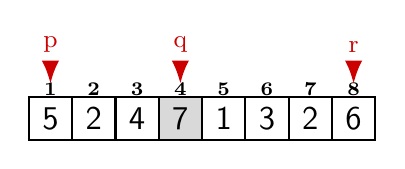
\begin{tikzpicture}[
						x=0.55cm, y=0.55cm, % Thu nhỏ xíu để vừa vặn
						cell/.style={
							draw=black, thick,
							minimum width=0.55cm, minimum height=0.55cm,
							font=\sffamily\large,
							anchor=center
						},
						idx/.style={
							font=\scriptsize\bfseries,
							anchor=south
						},
						ptr/.style={
							->, >=Latex, red!80!black, line width=1.2pt
						},
						ptr_label/.style={
							font=\small\color{red!80!black},
							anchor=south
						}
						]
						% Vẽ mảng
						\node[cell] (c1) at (1,0) {5};
						\node[cell] (c2) at (2,0) {2};
						\node[cell] (c3) at (3,0) {4};
						\node[cell, fill=gray!30] (c4) at (4,0) {7};
						\node[cell] (c5) at (5,0) {1};
						\node[cell] (c6) at (6,0) {3};
						\node[cell] (c7) at (7,0) {2};
						\node[cell] (c8) at (8,0) {6};
						
						% Chỉ số (1-8)
						\foreach \i in {1,...,8} {
							\node[idx] at (\i, 0.3) {\i};
						}
						
						% Mũi tên p, q, r
						\draw[ptr] (1, 1.3) -- (1, 0.8);
						\node[ptr_label] at (1, 1.3) {p};
						
						\draw[ptr] (4, 1.3) -- (4, 0.8);
						\node[ptr_label] at (4, 1.3) {q};
						
						\draw[ptr] (8, 1.3) -- (8, 0.8);
						\node[ptr_label] at (8, 1.3) {r};
						
					\end{tikzpicture}
				\end{adjustbox}
			\end{column}
			
		\end{columns}
		
		\begin{itemize}
			\item Lệnh gọi thực hiện thuật toán: \textcolor{black}{MERGE-SORT(A, 1, n)}
		\end{itemize}
		
	\end{frame}
	
	% ==================================================================
	% SLIDE 37: SẮP XẾP TRỘN (MERGE SORT) - THUẬT TOÁN MERGE
	% ==================================================================
	\begin{frame}[t]{1. SẮP XẾP TRỘN (MERGE SORT)}
		\textbf{\large 1.1. Sơ đồ thuật toán}
		
		\vspace{0.1cm}
		\begin{columns}[T, onlytextwidth]
			
			% --- CỘT TRÁI: MÃ GIẢ (Pseudocode) ---
			\begin{column}{0.55\textwidth}
				\scriptsize
				\textbf{MERGE(A, p, q, r)}
				\vspace{0.1cm}
				\begin{enumerate}
					\setlength\itemsep{0.2em} % Khoảng cách giữa các dòng
					\item Tính $n_1$ và $n_2$
					\item Sao $n_1$ phần tử đầu tiên vào $L[1 \dots n_1]$ và $n_2$ phần tử tiếp theo vào $R[1 \dots n_2]$
					\item $L[n_1 + 1] \leftarrow \infty$; \quad $R[n_2 + 1] \leftarrow \infty$
					\item $i \leftarrow 1$; \quad $j \leftarrow 1$
					\item \textbf{for} $k \leftarrow p$ \textbf{to} $r$ \textbf{do}
					\item \hspace{0.5cm} \textbf{if} $L[i] \le R[j]$
					\item \hspace{0.5cm} \textbf{then} $A[k] \leftarrow L[i]$
					\item \hspace{1.2cm} $i \leftarrow i + 1$
					\item \hspace{0.5cm} \textbf{else} $A[k] \leftarrow R[j]$
					\item \hspace{1.2cm} $j \leftarrow j + 1$
				\end{enumerate}
			\end{column}
			
			% --- CỘT PHẢI: HÌNH VẼ MINH HỌA ---
			\begin{column}{0.45\textwidth}
				\vspace{0.5cm}
				\begin{adjustbox}{width=1\linewidth}
					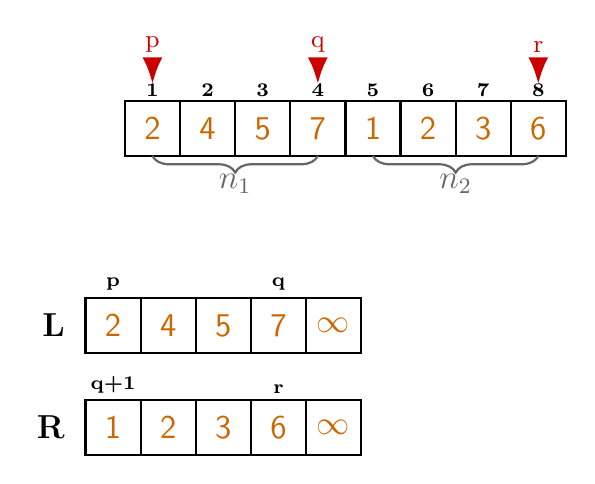
\begin{tikzpicture}[
						x=0.7cm, y=0.7cm,
						cell/.style={
							draw=black, thick,
							minimum width=0.7cm, minimum height=0.7cm,
							font=\sffamily\large\color{orange!80!black},
							anchor=center
						},
						idx_label/.style={
							font=\scriptsize\bfseries,
							anchor=south
						},
						ptr/.style={
							->, >=Latex, red!80!black, line width=1.5pt
						},
						ptr_text/.style={
							font=\small\color{red!80!black},
							anchor=south
						},
						brace_style/.style={
							decoration={brace, amplitude=6pt, mirror, raise=2pt},
							decorate, thick, gray!80!black
						}
						]
						% === MẢNG A (Top) ===
						% Data: 2, 4, 5, 7, 1, 2, 3, 6
						\foreach \val [count=\i] in {2, 4, 5, 7, 1, 2, 3, 6} {
							\node[cell] (a\i) at (\i, 0) {\val};
						}
						% Chỉ số nhỏ (1..8)
						\foreach \i in {1,...,8} {
							\node[idx_label] at (\i, 0.4) {\i};
						}
						
						% Mũi tên p, q, r
						\draw[ptr] (1, 1.2) -- (1, 0.8); \node[ptr_text] at (1, 1.2) {p};
						\draw[ptr] (4, 1.2) -- (4, 0.8); \node[ptr_text] at (4, 1.2) {q};
						\draw[ptr] (8, 1.2) -- (8, 0.8); \node[ptr_text] at (8, 1.2) {r};
						
						% Dấu ngoặc n1, n2
						\draw[brace_style] (1, -0.4) -- (4, -0.4) node[midway, yshift=-12pt, font=\large\color{red!80!black}] {$n_1$};
						\draw[brace_style] (5, -0.4) -- (8, -0.4) node[midway, yshift=-12pt, font=\large\color{red!80!black}] {$n_2$};
						
						% === MẢNG L (Left Subarray) ===
						\begin{scope}[yshift=-2.5cm, xshift=-0.5cm]
							\node[font=\large\bfseries, anchor=east] at (0.3, 0) {L};
							% Data: 2, 4, 5, 7, infinity
							\foreach \val [count=\i] in {2, 4, 5, 7} {
								\node[cell] (l\i) at (\i, 0) {\val};
							}
							\node[cell] (l5) at (5, 0) {$\infty$}; % Vô cực
							
							% Chỉ số p, q trên đầu mảng L
							\node[idx_label] at (1, 0.45) {p};
							\node[idx_label] at (4, 0.45) {q};
						\end{scope}
						
						% === MẢNG R (Right Subarray) ===
						\begin{scope}[yshift=-3.8cm, xshift=-0.5cm]
							\node[font=\large\bfseries, anchor=east] at (0.3, 0) {R};
							% Data: 1, 2, 3, 6, infinity
							\foreach \val [count=\i] in {1, 2, 3, 6} {
								\node[cell] (r\i) at (\i, 0) {\val};
							}
							\node[cell] (r5) at (5, 0) {$\infty$}; % Vô cực
							
							% Chỉ số q+1, r trên đầu mảng R
							\node[idx_label] at (1, 0.45) {q+1};
							\node[idx_label] at (4, 0.45) {r};
						\end{scope}
						
					\end{tikzpicture}
				\end{adjustbox}
			\end{column}
			
		\end{columns}
	\end{frame}
	
	\begin{frame}[t]{1. SẮP XẾP TRỘN (MERGE SORT)}
		\setlength{\leftmargini}{-1.2em}
		\small
		
		{\large \textbf{1.2. Thời gian tính}}
		
		\vspace{0.15cm}
		
		\begin{itemize}
			\item \textbf{Thời gian tính của bước trộn}
			\begin{itemize}
				\item Khởi tạo (tạo 2 mảng con tạm thời L và R):
				\begin{itemize}
					\item $\Theta(n_1+n_2)=\Theta(n)$
				\end{itemize}
				
				\vspace{0.1cm}
				
				\item Đưa các phần tử vào mảng kết quả (vòng lặp \textbf{for} cuối cùng):
				\begin{itemize}
					\item $n$ lần lặp, mỗi lần đòi hỏi thời gian hằng số $\Rightarrow\ \Theta(n)$
				\end{itemize}
				
				\vspace{0.1cm}
				
				\item Tổng cộng thời gian của trộn là:
				\begin{itemize}
					\item $\Theta(n)$
				\end{itemize}
			\end{itemize}
		\end{itemize}
		
	\end{frame}
	
	\begin{frame}[t]{1. SẮP XẾP TRỘN (MERGE SORT)}
		\setlength{\leftmargini}{-1.2em}
		\small
		
		{\large \textbf{1.2. Thời gian tính}}
		
		\begin{itemize}
			\item \textbf{Thời gian tính của sắp xếp trộn}
			\begin{itemize}
				\item Chia:
				\begin{itemize}
					\item tính $q$ như là giá trị trung bình của $p$ và $r$: $D(n)=\Theta(1)$
				\end{itemize}
				
				
				\item Trị:
				\begin{itemize}
					\item giải đệ qui $2$ bài toán con, mỗi bài toán kích thước $n/2 \Rightarrow 2T(n/2)$
				\end{itemize}
				
				\vspace{0.05cm}
				
				\item Tổ hợp:
				\begin{itemize}
					\item \textbf{TRỘN (MERGE)} trên các mảng con cỡ $n$ phần tử đòi hỏi thời gian $\Theta(n)$
					$\Rightarrow C(n)=\Theta(n)$
				\end{itemize}
			\end{itemize}
		\end{itemize}
		
		\[
		T(n)=
		\begin{cases}
			\Theta(1), & \text{nếu } n=1\\
			2T(n/2)+\Theta(n), & \text{nếu } n>1
		\end{cases}
		\]
		
		\vspace{0.15cm}
		
		{\color{red}\textbf{Suy ra theo định lý thợ:} $T(n)=\Theta(n\log n)$}
		
	\end{frame}
	
	% ==================================================================
	% SLIDE 40: VÍ DỤ MERGE SORT (SƠ ĐỒ CÂY - ĐÚNG MÀU)
	% ==================================================================
	\begin{frame}[t]{1. SẮP XẾP TRỘN (MERGE SORT)}
		\textbf{\large 1.3. Ví dụ}
		\vspace{-0.75cm}
		
		\begin{center}
			\begin{adjustbox}{width=0.55\textwidth}
				\begin{tikzpicture}[
					x=0.6cm, y=0.8cm, 
					cell/.style={
						draw=black, thick,
						minimum width=0.6cm, minimum height=0.6cm,
						font=\bfseries\large\color{orange}, % Số màu cam
						anchor=center
					},
					idx/.style={
						font=\tiny\color{blue}, % Chỉ số màu xanh
						anchor=south,
						yshift=1pt
					},
					div_arrow/.style={ % Mũi tên Chia (Đỏ đậm)
						->, >=Stealth, red!80!black, line width=1.5pt
					},
					merge_arrow/.style={ % Mũi tên Trộn (Xanh dương)
						->, >=Stealth, blue, line width=1.5pt
					},
					label_text/.style={ 
						font=\large\bfseries, 
						anchor=east, 
						align=right
					}
					]
					
					% ================= LEVEL 0: Mảng ban đầu =================
					\def\yA{0}
					\foreach \val [count=\i] in {8, 2, 9, 4, 5, 3, 1, 6} {
						\node[cell] (L0-\i) at (\i-4.5, \yA) {\val};
						\node[idx] at (L0-\i.north) {\i};
					}
					
					% ================= LEVEL 1: Divide 1 =================
					\def\yB{-2}
					\node[label_text, red!80!black] at (-7, \yB+0.5) {Divide}; % Nhãn đỏ
					
					% Left Block
					\foreach \val [count=\i] in {8, 2, 9, 4} {
						\node[cell] (L1L-\i) at (\i-7, \yB) {\val};
						\node[idx] at (L1L-\i.north) {\i};
					}
					% Right Block
					\foreach \val [count=\i] in {5, 3, 1, 6} {
						\node[cell] (L1R-\i) at (\i+2, \yB) {\val}; 
						\node[idx] at (L1R-\i.north) {\the\numexpr\i+4\relax};
					}
					
					\draw[div_arrow] (0, \yA-0.4) -- (-5, \yB+0.4); 
					\draw[div_arrow] (0, \yA-0.4) -- (4, \yB+0.4); 
					
					% ================= LEVEL 2: Divide 2 =================
					\def\yC{-4}
					\node[label_text, red!80!black] at (-9, \yC+0.5) {Divide}; % Nhãn đỏ
					
					% [8 2]
					\foreach \val [count=\i] in {8, 2} {
						\node[cell] (L2A-\i) at (\i-8.5, \yC) {\val};
						\node[idx] at (L2A-\i.north) {\i};
					}
					% [9 4]
					\foreach \val [count=\i] in {9, 4} {
						\node[cell] (L2B-\i) at (\i-4.5, \yC) {\val};
						\node[idx] at (L2B-\i.north) {\the\numexpr\i+2\relax};
					}
					% [5 3]
					\foreach \val [count=\i] in {5, 3} {
						\node[cell] (L2C-\i) at (\i+0.5, \yC) {\val};
						\node[idx] at (L2C-\i.north) {\the\numexpr\i+4\relax};
					}
					% [1 6]
					\foreach \val [count=\i] in {1, 6} {
						\node[cell] (L2D-\i) at (\i+4.5, \yC) {\val};
						\node[idx] at (L2D-\i.north) {\the\numexpr\i+6\relax};
					}
					
					\draw[div_arrow] (-5.5, \yB-0.4) -- (-8, \yC+0.4);
					\draw[div_arrow] (-4.5, \yB-0.4) -- (-3, \yC+0.4);
					\draw[div_arrow] (3.5, \yB-0.4) -- (1, \yC+0.4);
					\draw[div_arrow] (4.5, \yB-0.4) -- (6, \yC+0.4);
					
					% ================= LEVEL 3: 1 phần tử =================
					\def\yD{-6}
					\node[label_text, violet] at (-10, \yD) {1 phần tử}; % Nhãn tím
					
					% Vẽ 8 ô riêng lẻ
					\node[cell] (L3-1) at (-9, \yD) {8}; \node[idx] at (L3-1.north) {1};
					\node[cell] (L3-2) at (-7, \yD) {2}; \node[idx] at (L3-2.north) {2};
					\node[cell] (L3-3) at (-5, \yD) {9}; \node[idx] at (L3-3.north) {3};
					\node[cell] (L3-4) at (-3, \yD) {4}; \node[idx] at (L3-4.north) {4};
					\node[cell] (L3-5) at (0, \yD) {5}; \node[idx] at (L3-5.north) {5};
					\node[cell] (L3-6) at (2, \yD) {3}; \node[idx] at (L3-6.north) {6};
					\node[cell] (L3-7) at (4, \yD) {1}; \node[idx] at (L3-7.north) {7};
					\node[cell] (L3-8) at (6, \yD) {6}; \node[idx] at (L3-8.north) {8};
					
					\draw[div_arrow] (-8, \yC-0.4) -- (-9, \yD+0.4); \draw[div_arrow] (-7, \yC-0.4) -- (-7, \yD+0.4);
					\draw[div_arrow] (-4, \yC-0.4) -- (-5, \yD+0.4); \draw[div_arrow] (-3, \yC-0.4) -- (-3, \yD+0.4);
					\draw[div_arrow] (1, \yC-0.4) -- (0, \yD+0.4);   \draw[div_arrow] (2, \yC-0.4) -- (2, \yD+0.4);
					\draw[div_arrow] (5, \yC-0.4) -- (4, \yD+0.4);   \draw[div_arrow] (6, \yC-0.4) -- (6, \yD+0.4);
					
					% ================= LEVEL 4: Merge 1 =================
					\def\yE{-8}
					\node[label_text, blue] at (-10, \yE) {Merge}; % Nhãn xanh
					
					\node[cell] (L4A-1) at (-8.5, \yE) {2}; \node[cell] (L4A-2) at (-7.5, \yE) {8};
					\node[cell] (L4B-1) at (-4.5, \yE) {4}; \node[cell] (L4B-2) at (-3.5, \yE) {9};
					\node[cell] (L4C-1) at (0.5, \yE) {3};  \node[cell] (L4C-2) at (1.5, \yE) {5};
					\node[cell] (L4D-1) at (4.5, \yE) {1};  \node[cell] (L4D-2) at (5.5, \yE) {6};
					
					\draw[merge_arrow] (-9, \yD-0.4) -- (-8, \yE+0.4); \draw[merge_arrow] (-7, \yD-0.4) -- (-8, \yE+0.4);
					\draw[merge_arrow] (-5, \yD-0.4) -- (-4, \yE+0.4); \draw[merge_arrow] (-3, \yD-0.4) -- (-4, \yE+0.4);
					\draw[merge_arrow] (0, \yD-0.4) -- (1, \yE+0.4);   \draw[merge_arrow] (2, \yD-0.4) -- (1, \yE+0.4);
					\draw[merge_arrow] (4, \yD-0.4) -- (5, \yE+0.4);   \draw[merge_arrow] (6, \yD-0.4) -- (5, \yE+0.4);
					
					% ================= LEVEL 5: Merge 2 =================
					\def\yF{-10}
					\node[label_text, blue] at (-9, \yF) {Merge}; % Nhãn xanh
					
					\foreach \val [count=\i] in {2, 4, 8, 9} {
						\node[cell] (L5L-\i) at (\i-8.5, \yF) {\val};
						\ifnum\i=1 \node[idx] at (L5L-\i.north) {1}; \fi
						\ifnum\i=3 \node[idx] at (L5L-\i.north) {3}; \fi
						\ifnum\i=4 \node[idx] at (L5L-\i.north) {4}; \fi
					}
					\foreach \val [count=\i] in {1, 3, 5, 6} {
						\node[cell] (L5R-\i) at (\i+0.5, \yF) {\val};
						\ifnum\i=1 \node[idx] at (L5R-\i.north) {5}; \fi
						\ifnum\i=2 \node[idx] at (L5R-\i.north) {6}; \fi
						\ifnum\i=3 \node[idx] at (L5R-\i.north) {7}; \fi
						\ifnum\i=4 \node[idx] at (L5R-\i.north) {8}; \fi
					}
					
					\draw[merge_arrow] (-8, \yE-0.4) -- (-6, \yF+0.4);
					\draw[merge_arrow] (-4, \yE-0.4) -- (-6, \yF+0.4);
					\draw[merge_arrow] (1, \yE-0.4) -- (3, \yF+0.4);
					\draw[merge_arrow] (5, \yE-0.4) -- (3, \yF+0.4);
					
					% ================= LEVEL 6: Kết quả =================
					\def\yG{-12}
					\node[label_text, blue] at (-7, \yG) {Kết quả:}; % Nhãn xanh
					
					\foreach \val [count=\i] in {1, 2, 3, 4, 5, 6, 8, 9} {
						\node[cell] (L6-\i) at (\i-4.5, \yG) {\val};
						\node[idx] at (L6-\i.north) {\i};
					}
					
					\draw[merge_arrow] (-6, \yF-0.4) -- (0, \yG+0.4);
					\draw[merge_arrow] (3, \yF-0.4) -- (0, \yG+0.4);
					
				\end{tikzpicture}
			\end{adjustbox}
		\end{center}
	\end{frame}
	
	\subsection{Cài đặt thuật toán}
	
	% =========================
	% SLIDE 42: 2. CÀI ĐẶT THUẬT TOÁN (merge)
	% =========================
	\begin{frame}[t,fragile]{2. CÀI ĐẶT THUẬT TOÁN}
		\setlength{\leftmargini}{-1.2em}
		\small
		
		\vspace{0.1cm}
		
		\begin{tcolorbox}[
			width=\textwidth,
			height=0.70\textheight,
			colback=white,
			colframe=black!60,
			boxrule=0.6pt,
			arc=0pt,
			left=10pt,right=10pt,top=8pt,bottom=8pt
			]
			\begin{minted}[fontsize=\scriptsize,breaklines,linenos=false]{c}
				void merge(DataType A[], int first, int mid, int last){
					DataType tempA[MAX_SIZE];
					int first1 = first; int last1 = mid;
					int first2 = mid + 1; int last2 = last; int index = first1;
					
					for (; (first1 <= last1) && (first2 <= last2); ++index){
						if (A[first1] < A[first2]) { tempA[index] = A[first1]; ++first1; }
						else { tempA[index] = A[first2]; ++first2; }
					}
					for (; first1 <= last1; ++first1, ++index) tempA[index] = A[first1];
					for (; first2 <= last2; ++first2, ++index) tempA[index] = A[first2];
					for (index = first; index <= last; ++index) A[index] = tempA[index];
				} // end merge
			\end{minted}
			
			\vspace{0.15cm}
			{\color{red}\textbf{Chú ý: DataType: kiểu dữ liệu phần tử mảng.}}
		\end{tcolorbox}
		
	\end{frame}
	
	% =========================
	% SLIDE 43: 2. CÀI ĐẶT THUẬT TOÁN (mergesort)
	% =========================
	\begin{frame}[t,fragile]{2. CÀI ĐẶT THUẬT TOÁN}
		\setlength{\leftmargini}{-1.2em}
		\small
		
		\begin{itemize}
			\item Cài đặt mergesort
		\end{itemize}
		
		\vspace{-0.3cm}
		
		\begin{center}
			\begin{tcolorbox}[
				width=0.78\textwidth,
				height=0.58\textheight,
				colback=white,
				colframe=black!60,
				boxrule=0.6pt,
				arc=0pt,
				left=10pt,right=10pt,top=8pt,bottom=8pt
				]
				\begin{minted}[fontsize=\scriptsize,breaklines,linenos=false]{c}
					void mergesort(DataType A[], int first, int last) {
						if (first < last) {  // chia thành hai dãy con
							int mid = (first + last)/2;  // chỉ số điểm giữa
							
							// sắp xếp dãy con trái A[first..mid]
							mergesort(A, first, mid);
							
							// sắp xếp dãy con phải A[mid+1..last]
							mergesort(A, mid+1, last);
							
							// Trộn hai dãy con
							merge(A, first, mid, last);
						} // end if
					} // end mergesort
				\end{minted}
			\end{tcolorbox}
		\end{center}
		\begin{center}
			{\large \textcolor{blue}{\textbf{Lệnh gọi thực hiện }}\textcolor{red}{\textbf{mergesort(A,0,n-1)}}}
		\end{center}
		
	\end{frame}
	
		{\HUSTUseBackground{onelove.pdf}
		\begin{frame}
			\ifdefstring{\insertaspectratio}{169}{
				\HUSTCornerImage[0.14]{assets/logo/soict_vi_h.pdf}
				\placecontent{0.5cm}{0.33\paperheight}{0.85\paperwidth}{
					\color{\HUSTFrameTitleTextColor}\bfseries\fontsize{22pt}{30pt}\selectfont
					\inserttitle
				}
				\placecontent{0.5cm}{0.50\paperheight}{0.8\paperwidth}{
					\color{\HUSTFrameTitleTextColor}\fontsize{14pt}{14pt}\selectfont
					%Bài học
					\textbf{\large TUẦN 10: SẮP XẾP: Sắp xếp nhanh (quick sort)}\\
				}
			}{}
		\end{frame}
	}
	
	\section{Quick sort}
	\subsection{Sơ đồ tổng quát}
	
	% =========================
	% SLIDE 46: 1. SƠ ĐỒ TỔNG QUÁT (Quick Sort)
	% =========================
	\begin{frame}[t]{1. SƠ ĐỒ TỔNG QUÁT}
		\setlength{\leftmargini}{-1.2em}
		\small
		
		\begin{itemize}
			\item[$\triangleright$] Sơ đồ Quick Sort
		\end{itemize}
		
		\vspace{0.05cm}
		
		\begin{enumerate}
			\item \textcolor{blue}{Neo đệ qui:} Nếu dãy chỉ còn không quá 1 phần tử thì nó là dãy được sắp và trả lại ngay dãy này mà không phải làm gì cả.
			
			\vspace{0.1cm}
			
			\item \textcolor{blue}{Chia:}
			\begin{itemize}
				\item Chọn 1 phần tử trong dãy và gọi nó là \textcolor{red}{phần tử chốt $p$ (pivot)}.
				\item Chia dãy đã cho ra thành 2 dãy con:
				\begin{itemize}
					\item Dãy con trái (L) gồm những phần tử $\le$ phần tử chốt,
					\item Dãy con phải (R) gồm các phần tử $>$ phần tử chốt.
				\end{itemize}
				\item Thao tác này được gọi là \textcolor{red}{``Phân đoạn'' (Partition).}
			\end{itemize}
			
			\vspace{0.1cm}
			
			\item \textcolor{blue}{Trị:} Lặp lại một cách đệ qui thuật toán đối với 2 dãy con L và R.
			
			\vspace{0.1cm}
			
			\item \textcolor{blue}{Tổng hợp (Combine):} Dãy được sắp xếp là $L\ \textcolor{red}{p}\ R$.
		\end{enumerate}
		
	\end{frame}
	
	% ==================================================================
	% SLIDE 47: QUICK SORT - SƠ ĐỒ TỔNG QUÁT
	% ==================================================================
	\begin{frame}[t]{1. SƠ ĐỒ TỔNG QUÁT}
		\vspace{-0.45cm}
		
		\begin{center}
			\begin{adjustbox}{width=0.85\textwidth}
				\begin{tikzpicture}[
					font=\sffamily\bfseries,
					% Style cho các nhãn số
					num/.style={font=\sffamily\small},
					% Style cho Pivot (khoanh tròn xanh)
					pivot/.style={circle, draw=blue, thick, inner sep=2pt, font=\sffamily\small},
					% Style cho nhãn tập hợp (A, L, R)
					setlabel/.style={font=\Large\bfseries},
					% Style cho các mũi tên chỉ dẫn bên phải
					step_arrow/.style={
						->, >=Stealth, 
						draw=blue!60, line width=2pt,
						shorten >= 3pt, shorten <= 3pt
					},
					% Style cho text mô tả bên phải
					desc_text/.style={
						font=\large\color{orange!80!black}, 
						align=center
					}
					]
					
					% ================= LEVEL 1: Mảng A ban đầu =================
					\node[setlabel] at (-6, 0) {A};
					
					% Vẽ Elip bao quanh
					\draw (0, 0) ellipse (4.5cm and 0.8cm);
					
					% Các số bên trong (sắp xếp lộn xộn như hình)
					\node[num] at (-4.0, 0.1) {13};
					\node[num] at (-2.5, 0.4) {81};
					\node[num] at (-1.8, -0.3) {92};
					\node[num] at (-0.8, 0.3) {43};
					\node[num] at (0.2, 0.5) {31};
					\node[num] at (1.5, 0.5) {57};
					\node[num] at (3.0, 0.3) {75};
					\node[num] at (2.2, -0.3) {26};
					\node[num] at (3.8, 0.0) {0};
					
					% Pivot 65 ở giữa
					\node[pivot] (p1) at (0.0, -0.4) {65};
					
					% Mũi tên cong chọn Pivot
					\draw[->, >=Stealth, blue, line width=1pt] (5.5, 0.5) to[out=180, in=45] (p1.north east);
					\node[desc_text, anchor=west] at (5.6, 0.5) {Chọn pivot};
					
					
					% ================= Mũi tên bước 1 xuống bước 2 =================
					\draw[step_arrow] (6.5, 0.0) -- (6.5, -0.8);
					
					
					% ================= LEVEL 2: Phân đoạn (L, Pivot, R) =================
					\begin{scope}[yshift=-2.5cm]
						\node[setlabel] at (-5.5, 0.5) {L};
						\node[setlabel] at (1.8, 0.8) {R};
						
						% Tập L (nhỏ hơn 65)
						\draw (-2.5, 0) ellipse (2.2cm and 0.8cm);
						\node[num] at (-3.8, 0.3) {0};
						\node[num] at (-4.0, -0.2) {13};
						\node[num] at (-3.0, 0.1) {43};
						\node[num] at (-2.8, -0.5) {26};
						\node[num] at (-1.8, 0.4) {31};
						\node[num] at (-1.5, -0.4) {57};
						
						% Pivot
						\node[pivot] at (0.4, 0.0) {65};
						
						% Tập R (lớn hơn 65)
						\draw (3.5, 0) ellipse (2.2cm and 0.8cm);
						\node[num] at (2.5, -0.2) {92};
						\node[num] at (3.8, 0.4) {75};
						\node[num] at (4.8, 0.0) {81};
						
						% Text bên phải
						\node[desc_text, anchor=west] at (5.6, 0.5) {Phân đoạn A};
					\end{scope}
					
					
					% ================= Mũi tên bước 2 xuống bước 3 =================
					\draw[step_arrow] (6.5, -2.5) -- (6.5, -3.3);
					
					
					% ================= LEVEL 3: Gọi đệ quy (QuickSort L, R) =================
					\begin{scope}[yshift=-5.0cm]
						\node[setlabel] at (-5.5, 0.5) {L};
						\node[setlabel] at (1.8, 0.5) {R};
						
						% Tập L đã sắp xếp
						\draw (-2.5, 0) ellipse (2.5cm and 0.4cm);
						\node[num] at (-2.5, 0) {0 \ \ 13 \ \ 26 \ \ 31 \ \ 43 \ \ 57};
						
						% Pivot
						\node[pivot] at (0.8, 0.0) {65};
						
						% Tập R đã sắp xếp
						\draw (3.5, 0) ellipse (1.8cm and 0.4cm);
						\node[num] at (3.5, 0) {75 \ \ 81 \ \ 92};
						
						% Text bên phải
						\node[desc_text, anchor=west] at (5.6, 0.5) {QuickSort(L) và\\QuickSort(R)};
					\end{scope}
					
					
					% ================= Mũi tên bước 3 xuống bước 4 =================
					\draw[step_arrow] (6.5, -5.0) -- (6.5, -5.8);
					
					
					% ================= LEVEL 4: Kết quả (Mảng A đã sắp xếp) =================
					\begin{scope}[yshift=-6.5cm]
						\node[setlabel] at (-5.5, 0) {A};
						
						% Toàn bộ mảng A đã sắp xếp nối liền
						\draw (0.5, 0) ellipse (5.5cm and 0.4cm);
						\node[num] at (0.5, 0) {0 \ \ 13 \ \ 26 \ \ 31 \ \ 43 \ \ 57 \ \ \textbf{65} \ \ 75 \ \ 81 \ \ 92};
						
						% Text bên phải
						\node[desc_text, anchor=west] at (6.1, 0) {A được sắp};
					\end{scope}
					
				\end{tikzpicture}
			\end{adjustbox}
		\end{center}
	\end{frame}
	
	% =========================
	% SLIDE 48: 1. SƠ ĐỒ TỔNG QUÁT (QuickSort + Partition)
	% =========================
	\begin{frame}[t,fragile]{1. SƠ ĐỒ TỔNG QUÁT}
		\setlength{\leftmargini}{-1.2em}
		\small
		
		\vspace{-0.35cm}
		
		\begin{columns}[T,totalwidth=\textwidth]
			% ---- Left: PARTITION ----
			\begin{column}{0.45\textwidth}
				\begin{tcolorbox}[
					width=\linewidth,
					height=0.70\textheight,
					colback=white,
					colframe=blue!60,
					boxrule=0.8pt,
					arc=0pt,
					left=-50pt,right=8pt,top=0pt,bottom=8pt
					]
					\begin{minted}[fontsize=\scriptsize,linenos=false]{c}
						PARTITION(a, L, R, q) {
							
							pivot = a[q]; SWAP(a[q], a[R]); nq = L;
							
							for i = L to R-1 do {
								
								if a[i] < pivot then {
									
									SWAP(a[i], a[nq]); nq = nq + 1;
									
								}
								
							}
							
							SWAP(a[nq], a[R]);
							
							return nq;
						}
					\end{minted}
				\end{tcolorbox}
			\end{column}
			
			% ---- Right: QUICK-SORT ----
			\begin{column}{0.45\textwidth}
				\begin{tcolorbox}[
					width=\linewidth,
					height=0.70\textheight,
					colback=white,
					colframe=blue!60,
					boxrule=0.8pt,
					arc=0pt,
					left=-40pt,right=8pt,top=0pt,bottom=8pt
					]
					\begin{minted}[fontsize=\scriptsize,breaklines,linenos=false]{c}
						QUICK-SORT(a, L, R) {
							
							if L >= R then return;
							
							q = select(L,R);
							
							q = PARTITION(a, L, R, q);
							
							QUICK-SORT(a, L, q-1);
							
							QUICK-SORT(a, q+1, R);
							
						}
					\end{minted}
				\end{tcolorbox}
			\end{column}
		\end{columns}
		
	\end{frame}
	
	% =========================
	% SLIDE 49: 1. SƠ ĐỒ TỔNG QUÁT (Độ phức tạp tính toán)
	% =========================
	\begin{frame}[t]{1. SƠ ĐỒ TỔNG QUÁT}
		\setlength{\leftmargini}{-1.2em}
		\small
		
		\begin{itemize}
			\item Độ phức tạp tính toán
			\begin{itemize}
				\item Tình huống tồi nhất $O(n^2)$
				\item Tình huống tốt nhất $O(n\log n)$
				\item Tình huống trung bình: chọn pivot ngẫu nhiên, thời gian tính $O(n\log n)$
			\end{itemize}
		\end{itemize}
		
	\end{frame}
	
	
	
	{\HUSTUseBackground{onelove.pdf}
		\begin{frame}
			\ifdefstring{\insertaspectratio}{169}{
				\HUSTCornerImage[0.14]{assets/logo/soict_vi_h.pdf}
				\placecontent{0.5cm}{0.33\paperheight}{0.85\paperwidth}{
					\color{\HUSTFrameTitleTextColor}\bfseries\fontsize{22pt}{30pt}\selectfont
					\inserttitle
				}
				\placecontent{0.5cm}{0.50\paperheight}{0.8\paperwidth}{
					\color{\HUSTFrameTitleTextColor}\fontsize{14pt}{14pt}\selectfont
					%Bài học
					\textbf{\large TUẦN 10: SẮP XẾP: Sắp xếp vun đống (heap sort)}\\
				}
			}{}
		\end{frame}
	}
	
	\section{heap sort}
	\subsection{Cấu trúc dữ liệu đống}
	
	% ==================================================================
	% SLIDE 52: CẤU TRÚC DỮ LIỆU ĐỐNG (HEAP)
	% ==================================================================
	\begin{frame}[t]{1. CẤU TRÚC DỮ LIỆU ĐỐNG}
		\setlength{\leftmargini}{-0.5em}
		
		\begin{itemize}
			\item \textcolor{red!80!black}{\textbf{Định nghĩa:}} \textbf{Đống (heap)} là cây nhị phân \textit{hoàn chỉnh} có 2 tính chất:
			\begin{itemize}
				\item \textbf{Tính cấu trúc:} tất cả các mức đều là đầy, ngoại trừ mức cuối cùng, mức cuối được điền từ trái sang phải.
				\item \textbf{Tính có thứ tự hay tính chất đống:} với mỗi nút $x$
				\[ Parent(x) \ge x. \]
			\end{itemize}
			\item Cây được cài đặt bởi mảng A[i] có độ dài $length[A]$. Số lượng phần tử là $heapsize[A]$
		\end{itemize}
		
		\begin{columns}[T, onlytextwidth]
			% --- CỘT TRÁI: Hình vẽ cây Heap ---
			\begin{column}{0.4\textwidth}
				\centering
				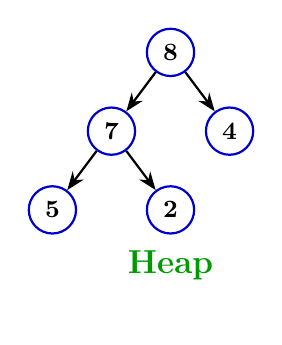
\begin{tikzpicture}[
					level distance=1.0cm,
					sibling distance=1.5cm,
					every node/.style={
						circle, draw=blue!80!black, thick,
						inner sep=2pt, minimum size=0.6cm,
						font=\small\bfseries
					},
					edge from parent/.style={
						draw, black, thick, ->, >=Stealth
					}
					]
					% Vẽ cây: 8 -> (7, 4) -> 7 -> (5, 2)
					\node {8}
					child { node {7}
						child { node {5} }
						child { node {2} }
					}
					child { node {4} };
					
					% Nhãn "Heap" màu xanh lá
					\node[draw=none, text=green!60!black, font=\large\bfseries, yshift=-3.2cm] at (0,0.5) {Heap};
				\end{tikzpicture}
			\end{column}
			
			% --- CỘT PHẢI: Giải thích ---
			\begin{column}{0.6\textwidth}
				\vspace{0.5cm}
				\large
				\textcolor{blue!80!black}{Từ tính chất đống suy ra:}
				
				\vspace{0.1cm}
				\textcolor{red}{\textbf{“Gốc chứa phần tử lớn nhất của đống!”}}
				
				\vspace{0.3cm}
				\textcolor{blue!80!black}{Như vậy có thể nói:}
				
				\vspace{0.1cm}
				\textcolor{red}{Đống là cây nhị phân được điền theo thứ tự}
			\end{column}
		\end{columns}
	\end{frame}
	
	% ==================================================================
	% SLIDE 53: BIỂU DIỄN ĐỐNG BỞI MẢNG
	% ==================================================================
	\begin{frame}[t]{1. CẤU TRÚC DỮ LIỆU ĐỐNG}
		\setlength{\leftmargini}{-0.5em}
		\vspace{-0.2cm}
		
		\begin{columns}[T, onlytextwidth]
			% --- CỘT TRÁI: LÝ THUYẾT ---
			\begin{column}{0.45\textwidth}
				\textbf{\large $\gg$ Biểu diễn đống bởi mảng}
				\begin{itemize}
					\item Đống có thể cất giữ trong mảng A.
					\begin{itemize}
						\item Gốc của cây là A[1]
						\item Con trái của A[i] là A[$2*i$]
						\item Con phải của A[i] là A[$2*i + 1$]
						\item Cha của A[i] là A[$\lfloor i/2 \rfloor$]
						\item Heapsize[A] $\le$ length[A]
					\end{itemize}
					\vspace{0.2cm}
					\item Các phần tử trong mảng con $A[(\lfloor n/2 \rfloor + 1) .. n]$ là các lá
				\end{itemize}
			\end{column}
			
			% --- CỘT PHẢI: HÌNH VẼ MINH HỌA ---
			\begin{column}{0.50\textwidth}
				\centering
				
				% --- PHẦN 1: MẢNG VỚI CÁC ĐƯỜNG CONG ---
				\begin{adjustbox}{width=0.8\linewidth}
					\begin{tikzpicture}[
						x=0.6cm, y=0.6cm,
						cell/.style={draw, thick, minimum size=0.6cm, font=\small},
						link/.style={->, >=Stealth, thin, bend left=50},
						idx/.style={font=\tiny, color=gray}
						]
						% Vẽ mảng dữ liệu: 16 14 10 8 7 9 3 2 4 1
						\foreach \val [count=\i] in {16, 14, 10, 8, 7, 9, 3, 2, 4, 1} {
							\node[cell] (c\i) at (\i, 0) {\val};
							\node[idx, above=0.05cm of c\i] {\i};
						}
						
						% Vẽ các đường cong quan hệ cha-con
						% 1 -> 2,3
						\draw (c1.north) to[bend left=60] (c2.north);
						\draw (c1.north) to[bend left=70] (c3.north);
						% 2 -> 4,5
						\draw (c2.north) to[bend left=60] (c4.north);
						\draw (c2.north) to[bend left=70] (c5.north);
						% 3 -> 6,7
						\draw (c3.north) to[bend left=60] (c6.north);
						\draw (c3.north) to[bend left=70] (c7.north);
						% 4 -> 8,9 (Vẽ phía dưới cho đỡ rối, hoặc phía trên tùy ý, hình mẫu vẽ tất cả phía trên nhưng khá rối, ta vẽ xen kẽ hoặc dùng styles khác nhau)
						% Để giống hình mẫu nhất, ta vẽ phía dưới cho lớp con sâu hơn
						\draw (c4.south) to[bend right=60] (c8.south);
						\draw (c4.south) to[bend right=70] (c9.south);
						% 5 -> 10
						\draw (c5.south) to[bend right=60] (c10.south);
						
						\node[font=\itshape\footnotesize, below=0.8cm of c5] {Mảng đầu vào};
					\end{tikzpicture}
				\end{adjustbox}
				
				\vspace{0.5cm}
				
				% --- PHẦN 2: CÂY NHỊ PHÂN ---
			\begin{adjustbox}{width=1\linewidth}
				\begin{tikzpicture}[
					% --- TINH CHỈNH KÍCH THƯỚC ---
					level distance=1.0cm,            % Chiều dọc hẹp lại (mặc định thường 1.5cm -> giảm còn 1.0cm)
					level 1/.style={sibling distance=6.0cm}, % Level 1 xòe rất rộng
					level 2/.style={sibling distance=3.0cm}, % Level 2 xòe vừa
					level 3/.style={sibling distance=1.5cm}, % Level 3 (lá)
					% -----------------------------
					every node/.style={
						circle, draw, thick, 
						inner sep=0pt, minimum size=0.7cm, 
						font=\bfseries
					},
					edge from parent/.style={draw, thick},
					% Style cho số chỉ mục nhỏ (index) bên trên
					idx_label/.style={
						draw=none, font=\scriptsize\color{black!70}, above=1pt
					}
					]
					% Gốc (index 1)
					\node[label={[idx_label]90:1}] {16}
					% Nhánh trái (index 2)
					child { 
						node[label={[idx_label]90:2}] {14}
						% Con của 14: 8 (trái) và 7 (phải)
						child { 
							node[label={[idx_label]135:4}] {8} 
							child { node[label={[idx_label]90:8}] {2} }
							child { node[label={[idx_label]90:9}] {4} }
						}
						child { 
							node[label={[idx_label]45:5}] {7}
							child { node[label={[idx_label]90:10}] {1} }
							child[missing] % Khuyết con phải của 7
						}
					}
					% Nhánh phải (index 3)
					child { 
						node[label={[idx_label]90:3}] {10}
						child { node[label={[idx_label]90:6}] {9} }
						child { node[label={[idx_label]90:7}] {3} }
					};
					
					% Chú thích dưới cây
					\node[draw=none, rectangle, below=0.2cm of current bounding box, font=\itshape\small] {Đống tương ứng của mảng};
				\end{tikzpicture}
			\end{adjustbox}
				
			\end{column}
		\end{columns}
	\end{frame}
	
	
	% ==================================================================
	% SLIDE 54: VÍ DỤ 1 - ĐỐNG
	% ==================================================================
	\begin{frame}[t]{1. CẤU TRÚC DỮ LIỆU ĐỐNG}
		\textbf{\large $\gg$ \ Ví dụ 1: Đống}
		\begin{columns}[T, onlytextwidth]
			% --- CỘT TRÁI: Cây Heap ---
			\begin{column}{0.5\textwidth}
				\centering
				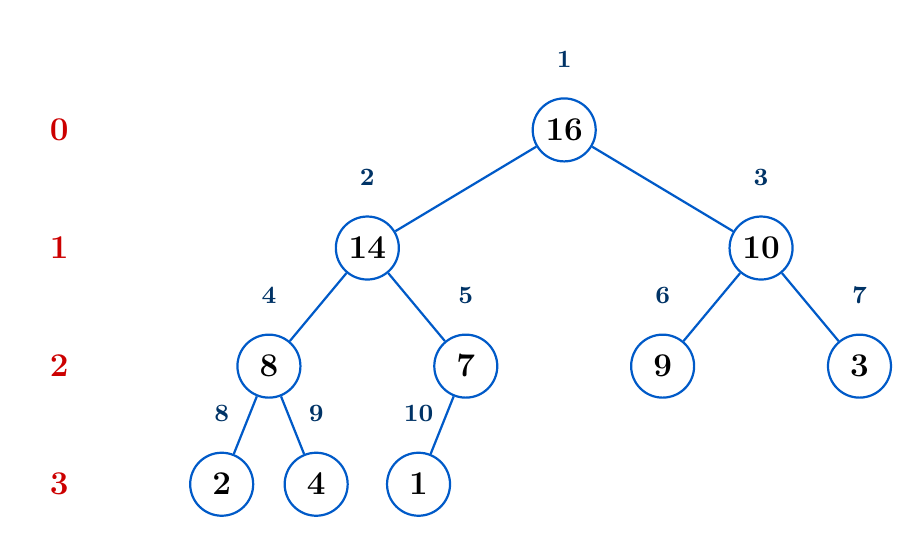
\begin{tikzpicture}[
					level distance=1.5cm,
					level 1/.style={sibling distance=5cm},
					level 2/.style={sibling distance=2.5cm},
					level 3/.style={sibling distance=1.2cm},
					every node/.style={
						circle, draw=codeblue, thick, 
						inner sep=0pt, minimum size=0.8cm, 
						font=\bfseries\large
					},
					edge from parent/.style={draw=codeblue, thick},
					% Style cho chỉ số index nhỏ màu xanh dương đậm trên đầu node
					idx_label/.style={
						draw=none, font=\bfseries\small\color{HUSTBlue}, above=2pt
					},
					% Style cho nhãn Level đỏ bên trái
					level_label/.style={
						draw=none, font=\bfseries\large\color{red!80!black}, 
						anchor=east, xshift=-2cm
					}
					]
					% Gốc (Level 0)
					\node[label={[idx_label]90:1}] (root) {16}
					child { 
						node[label={[idx_label]90:2}] (n2) {14}
						child { 
							node[label={[idx_label]90:4}] (n4) {8} 
							child { node[label={[idx_label]90:8}] (n8) {2} }
							child { node[label={[idx_label]90:9}] (n9) {4} }
						}
						child { 
							node[label={[idx_label]90:5}] (n5) {7}
							child { node[label={[idx_label]90:10}] (n10) {1} }
							child[missing] 
						}
					}
					child { 
						node[label={[idx_label]90:3}] (n3) {10}
						child { node[label={[idx_label]90:6}] (n6) {9} }
						child { node[label={[idx_label]90:7}] (n7) {3} }
					};
					
					% Vẽ các nhãn Level 0, 1, 2, 3 bên trái
					% Dùng tọa độ y của các node để căn dòng
					\node[level_label] at (-4, 0) {0};    % Ngang hàng root
					\node[level_label] at (-4, -1.5) {1}; % Ngang hàng con cấp 1
					\node[level_label] at (-4, -3.0) {2}; % Ngang hàng con cấp 2
					\node[level_label] at (-4, -4.5) {3}; % Ngang hàng con cấp 3 (lá)
					
				\end{tikzpicture}
			\end{column}
			
			% --- CỘT PHẢI: Công thức & Mảng ---
		% --- CỘT PHẢI: Công thức & Mảng (ĐÃ SỬA LỖI MATRIX) ---
		\begin{column}{0.4\textwidth}
			% 1. Công thức
			\vspace{-0.5cm}
			\begin{itemize}
				\item[] \textcolor{red!80!black}{parent(i) = $\lfloor i/2 \rfloor$}
				\item[] \textcolor{red!80!black}{left-child(i) = $2i$}
				\item[] \textcolor{red!80!black}{right-child(i) = $2i + 1$}
			\end{itemize}
			
			\vspace{3.7cm}
			\begin{adjustbox}{right}
				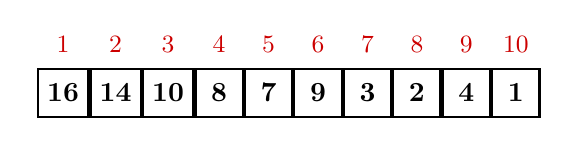
\begin{tikzpicture}[
					cell/.style={
						draw, thick, minimum width=0.6cm, minimum height=0.6cm,
						font=\bfseries, anchor=center
					},
					idx/.style={
						font=\small\color{red}, below=2pt 
					}
					]
					% SỬA LẠI PHẦN NÀY:
					\matrix (m) [
					matrix of nodes, 
					nodes={cell}, 
					column sep=0pt, 
					row sep=0pt,
					ampersand replacement=\& % <--- THÊM DÒNG NÀY
					] {
						% Thay dấu & bằng \&
						16 \& 14 \& 10 \& 8 \& 7 \& 9 \& 3 \& 2 \& 4 \& 1 \\
					};
					
					% Đánh số chỉ số index
					\foreach \i in {1,...,10} {
						\node[font=\small\color{red!80!black}, above=2pt] at (m-1-\i.north) {\i};
					}
				\end{tikzpicture}
			\end{adjustbox}
		\end{column}
		\end{columns}
	\end{frame}
	
	% =========================
	% SLIDE 55: 1. CẤU TRÚC DỮ LIỆU ĐỐNG (Hai dạng đống)
	% =========================
	\begin{frame}[t]{1. CẤU TRÚC DỮ LIỆU ĐỐNG}
		\setlength{\leftmargini}{-1.2em}
		\small
		
		\begin{itemize}
			\item[$\triangleright$] Hai dạng đống
		\end{itemize}
		
		\vspace{0.05cm}
		
		\begin{itemize}
			\item \textbf{Đống max - Max-heaps} (Phần tử lớn nhất ở gốc), có tính chất \textit{max-heap}:
			\begin{itemize}
				\item với mọi nút $i$, ngoại trừ gốc:
			\end{itemize}
		\end{itemize}
		
		\vspace{-0.05cm}
		\[
		A[\text{parent}(i)] \ge A[i]
		\]
		
		\vspace{0.05cm}
		
		\begin{itemize}
			\item \textbf{Đống min - Min-heaps} (phần tử nhỏ nhất ở gốc), có tính chất \textit{min-heap}:
			\begin{itemize}
				\item với mọi nút $i$, ngoại trừ gốc:
			\end{itemize}
		\end{itemize}
		
		\vspace{-0.05cm}
		\[
		A[\text{parent}(i)] \le A[i]
		\]
		
		\vspace{0.15cm}
		
		\begin{itemize}
			\item \textcolor{red}{Phần dưới đây ta sẽ chỉ xét đống max (max-heap). Đống min được xét hoàn toàn tương tự.}
		\end{itemize}
		
	\end{frame}
	
	% ==================================================================
	% SLIDE 56: HAI DẠNG ĐỐNG - VÍ DỤ ĐỐNG CỰC ĐẠI
	% ==================================================================
	\begin{frame}[t]{1. CẤU TRÚC DỮ LIỆU ĐỐNG}
		\setlength{\leftmargini}{-1.2em}
		\textbf{\large $\gg$ \ Hai dạng đống}
		
		\begin{itemize}
			\item Nút mới được bổ sung vào mức đáy (từ trái sang phải)
			\item Các nút được loại bỏ khỏi mức đáy (từ phải sang trái)
		\end{itemize}

		\begin{center}
			\begin{tikzpicture}[
				level distance=1.2cm,
				level 1/.style={sibling distance=5cm},
				level 2/.style={sibling distance=2.5cm},
				level 3/.style={sibling distance=1.2cm},
				every node/.style={
					circle, draw=black, thick, 
					inner sep=0pt, minimum size=0.7cm, 
					font=\small\bfseries
				},
				edge from parent/.style={draw=black, thin}
				]
				% Vẽ cây: 50 -> (24, 30)
				% 24 -> (20, 21), 30 -> (18, 3)
				% 20 -> (12, 5), 21 -> (6, missing)
				
				\node {50}
				child { 
					node {24}
					child { 
						node {20} 
						child { node {12} }
						child { node {5} }
					}
					child { 
						node {21}
						child { node {6} }
						child[missing] % Khuyết con phải của 21
					}
				}
				child { 
					node {30}
					child { node {18} }
					child { node {3} }
				};
				
				% Nhãn caption phía dưới
				\node[draw=none, rectangle, below=0.1cm of current bounding box, font=\itshape\small] 
				{Ví dụ đống cực đại};
				
			\end{tikzpicture}
		\end{center}
	\end{frame}
	
	% =========================
	% SLIDE 57: 1. CẤU TRÚC DỮ LIỆU ĐỐNG (Các phép toán đối với đống)
	% =========================
	\begin{frame}[t]{1. CẤU TRÚC DỮ LIỆU ĐỐNG}
		\setlength{\leftmargini}{-1.2em}
		\small
		
		{\large\textbf{Các phép toán đối với đống}}
		
		\vspace{0.35cm}
		
		\begin{itemize}
			\item Khôi phục tính chất max-heap (Vun lại đống)
			\begin{itemize}
				\item \textcolor{blue}{Max-Heapify}
			\end{itemize}
			
			\vspace{0.35cm}
			
			\item Tạo max-heap từ một mảng không được sắp xếp
			\begin{itemize}
				\item \textcolor{blue}{Build-Max-Heap}
			\end{itemize}
		\end{itemize}
		
	\end{frame}
	
	% ==================================================================
	% SLIDE 57: VUN ĐỐNG (HEAPIFY)
	% ==================================================================
	\begin{frame}[t]{2. VUN ĐỐNG (HEAPIFY)}
		\setlength{\leftmargini}{-1.2em}
		\small
		
		\begin{columns}[T, onlytextwidth]
			% --- CỘT TRÁI: LÝ THUYẾT ---
			\begin{column}{0.55\textwidth}
				\large
				\textbf{\textcolor{blue!80!black}{Thủ tục Max-Heapify(A, i)}}
				
				\vspace{0.3cm}
				\begin{itemize}
					\setlength\itemsep{0.5em}
					\item \textbf{Input:} Mảng A và chỉ số i.
					\item \textbf{Giả thiết:} Các cây con gốc tại \textcolor{red}{$Left(i)$} và \textcolor{red}{$Right(i)$} đã là đống cực đại.
					\item \textbf{Vấn đề:} Phần tử tại $A[i]$ có thể nhỏ hơn các con của nó $\rightarrow$ vi phạm tính chất đống.
					\item \textbf{Công việc:} "Thả trôi" giá trị tại $A[i]$ xuống (trong cây đống) để phần tử tại cây con gốc $i$ tuân thủ tính chất đống.
				\end{itemize}
			\end{column}
			
			% --- CỘT PHẢI: HÌNH MINH HỌA ---
			\begin{column}{0.45\textwidth}
				\centering
				\begin{adjustbox}{width=0.95\linewidth}
					\begin{tikzpicture}[
						level distance=1.3cm,
						level 1/.style={sibling distance=3.5cm},
						level 2/.style={sibling distance=1.8cm},
						every node/.style={
							circle, draw=codeblue, thick, 
							inner sep=0pt, minimum size=0.8cm, 
							font=\bfseries\large
						},
						edge from parent/.style={draw=black, thick},
						% Style cho node vi phạm (màu đỏ)
						bad_node/.style={
							fill=red!20, draw=red, text=red!80!black
						},
						% Mũi tên hoán đổi
						swap_arrow/.style={
							->, >=Stealth, red, line width=1.5pt, bend right=45, dashed
						}
						]
						% Vẽ cây ví dụ:
						% Gốc là 4 (vi phạm vì nhỏ hơn 14 và 7)
						% Trái: 14 (có con 2, 8)
						% Phải: 7 (có con 1)
						
						\node[bad_node] (n1) {4}
						child { 
							node (n2) {14}
							child { node (n4) {2} }
							child { node (n5) {8} }
						}
						child { 
							node (n3) {7}
							child { node (n6) {1} }
							child[missing] 
						};
						
						% Chỉ số i bên cạnh gốc
						\node[draw=none, right=0.1cm of n1, font=\large\bfseries\color{black}] {i};
						
						% Chú thích
						\node[draw=none, rectangle, below=3.5cm, font=\itshape\color{blue!80!black}, align=center] 
						{Nút i vi phạm tính chất đống};
						
					\end{tikzpicture}
				\end{adjustbox}
			\end{column}
		\end{columns}
	\end{frame}
	% ==================================================================
	% SLIDE: VÍ DỤ 2 - HEAPIFY (Đã chỉnh sửa theo yêu cầu)
	% ==================================================================
	\begin{frame}[t]{1. CẤU TRÚC DỮ LIỆU ĐỐNG}
		\textbf{\large $\gg$ \ Ví dụ 2}
		
		\vspace{-0.6cm} % Kéo hình lên một chút
		
		\begin{center}
			% YÊU CẦU: Resize về 0.75\textwidth
			\resizebox{0.75\textwidth}{!}{
				\begin{tikzpicture}[
					level distance=1.2cm,
					level 1/.style={sibling distance=3.5cm},
					level 2/.style={sibling distance=1.8cm},
					level 3/.style={sibling distance=1.0cm},
					mynode/.style={
						circle, draw=black, thick, 
						minimum size=0.7cm, inner sep=0pt,
						font=\small\bfseries
					},
					focusnode/.style={
						mynode, line width=1.8pt
					},
					idx/.style={
						font=\tiny, color=black!70, above=1pt
					},
					edge from parent/.style={draw=black, thick}
					]
					
					% --- CÂY 1 (TRÁI): A[2] vi phạm ---
					\begin{scope}[local bounding box=tree1]
						\node[mynode, label={[idx]90:1}] {16}
						child { 
							node[focusnode, label={[idx]90:2}, label={[font=\small\itshape]180:$i$}] {4}
							child { 
								node[mynode, label={[idx]90:4}] {14} 
								child { node[mynode, label={[idx]90:8}] {2} }
								child { node[mynode, label={[idx]90:9}] {8} }
							}
							child { 
								node[mynode, label={[idx]90:5}] {7}
								child { node[mynode, label={[idx]90:10}] {1} }
								child[missing] 
							}
						}
						child { 
							node[mynode, label={[idx]90:3}] {10}
							child { node[mynode, label={[idx]90:6}] {9} }
							child { node[mynode, label={[idx]90:7}] {3} }
						};
						\node[below=0.1cm of tree1, blue, font=\bfseries] {A[2] vi phạm tính chất đống};
					\end{scope}
					
					% --- TEXT 1: Giữa cây 1 và 2 ---
					\node[red, font=\large\bfseries] at (5, -1.5) {A[2] $\leftrightarrow$ A[4]};
					
					% --- CÂY 2 (PHẢI): A[4] vi phạm ---
					\begin{scope}[xshift=10cm, local bounding box=tree2]
						\node[mynode, label={[idx]90:1}] {16}
						child { 
							node[mynode, label={[idx]90:2}] {14} 
							child { 
								node[focusnode, label={[idx]90:4}, label={[font=\small\itshape]180:$i$}] {4} 
								child { node[mynode, label={[idx]90:8}] {2} }
								child { node[mynode, label={[idx]90:9}] {8} }
							}
							child { 
								node[mynode, label={[idx]90:5}] {7}
								child { node[mynode, label={[idx]90:10}] {1} }
								child[missing] 
							}
						}
						child { 
							node[mynode, label={[idx]90:3}] {10}
							child { node[mynode, label={[idx]90:6}] {9} }
							child { node[mynode, label={[idx]90:7}] {3} }
						};
						\node[below=0.1cm of tree2, blue, font=\bfseries] {A[4] vi phạm};
					\end{scope}
					
					% --- CÂY 3 (DƯỚI): Đẩy lên cao hơn (yshift = -5.2cm thay vì -7.5cm) ---
					\begin{scope}[xshift=5cm, yshift=-5.2cm, local bounding box=tree3]
						\node[mynode, label={[idx]90:1}] {16}
						child { 
							node[mynode, label={[idx]90:2}] {14} 
							child { 
								node[mynode, label={[idx]90:4}] {8} 
								child { node[mynode, label={[idx]90:8}] {2} }
								child { node[focusnode, label={[idx]90:9}, label={[font=\small\itshape]135:$i$}] {4} }
							}
							child { 
								node[mynode, label={[idx]90:5}] {7}
								child { node[mynode, label={[idx]90:10}] {1} }
								child[missing] 
							}
						}
						child { 
							node[mynode, label={[idx]90:3}] {10}
							child { node[mynode, label={[idx]90:6}] {9} }
							child { node[mynode, label={[idx]90:7}] {3} }
						};
						\node[below=0.1cm of tree3, blue, font=\bfseries] {Tính chất đống được khôi phục};
					\end{scope}
					
					% --- TEXT 2: Chuyển sang cạnh trái cây 3 ---
					% Đặt tại vị trí (0.5, -5.2) tức là bên trái root của cây 3
					\node[red, font=\large\bfseries, anchor=east] at (2.5, -5.2) {A[4] $\leftrightarrow$ A[9]};
					
				\end{tikzpicture}
			}
		\end{center}
	\end{frame}
	
	% =========================
	% SLIDE 60 
	% =========================
	\begin{frame}[t,fragile]{1. CẤU TRÚC DỮ LIỆU ĐỐNG}
		\setlength{\leftmargini}{-1.2em}
		\small
		
		\begin{columns}[T,totalwidth=\textwidth]
			% ---------------- Left block ----------------
			\begin{column}{0.55\textwidth}
				{\large\textbf{Thuật toán khôi phục tính chất đống}}
				
				\vspace{0.2cm}
				
				\begin{itemize}
					\item \textcolor{blue}{\textbf{Giả thiết:}}
					\begin{itemize}
						\item \textcolor{blue}{Cả hai cây con trái và phải của $i$\\ đều là max-heaps}
						\item \textcolor{blue}{$A[i]$ có thể bé hơn các con của nó}
					\end{itemize}
				\end{itemize}

				\begin{center}
					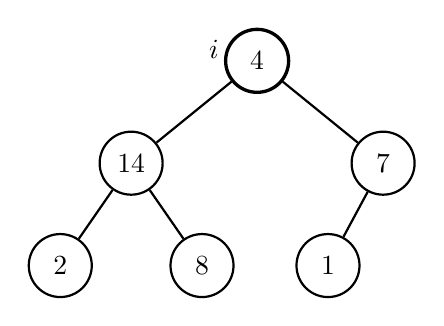
\begin{tikzpicture}[
						node/.style={circle, draw=black, thick, minimum size=8mm, inner sep=0pt},
						root/.style={node, line width=1.2pt},
						edge/.style={thick}
						]
						\node[root] (r) at (0,0) {4};
						\node[node] (l)  at (-1.6,-1.3) {14};
						\node[node] (rr) at ( 1.6,-1.3) {7};
						\node[node] (ll) at (-2.5,-2.6) {2};
						\node[node] (lr) at (-0.7,-2.6) {8};
						\node[node] (rl) at ( 0.9,-2.6) {1};
						
						\draw[edge] (r) -- (l);
						\draw[edge] (r) -- (rr);
						\draw[edge] (l) -- (ll);
						\draw[edge] (l) -- (lr);
						\draw[edge] (rr) -- (rl);
						
						\node[font=\itshape] at (-0.55,0.15) {$i$};
					\end{tikzpicture}
				\end{center}
			\end{column}
			
			% ---------------- Right block (MINTED bình thường) ----------------
			\begin{column}{0.45\textwidth}
				\begin{tcolorbox}[
					width=\linewidth,
					height=0.73\textheight,
					colback=white,
					colframe=black!70,
					boxrule=0.7pt,
					arc=0pt,
					left=10pt,right=10pt,top=8pt,bottom=8pt
					]
					{\Large \underline{\textbf{Max-Heapify(A,i,n)}}}
					
					\vspace{0.15cm}
					{\itshape // n = heapsize[A]}
					
				\begin{minted}[
					fontsize=\scriptsize,
					linenos=false,
					escapeinside=||,
					gobble=4
					]{text}
					1. |$l \leftarrow \textit{left-child}(i)$|
					2. |$r \leftarrow \textit{right-child}(i)$|
					3. |$\mathbf{if}\ (l \le n)\ \text{and}\ (A[l] > A[i])$|
					4.     |$\mathbf{then}\ \textit{largest} \leftarrow l$|
					5.     |$\mathbf{else}\ \textit{largest} \leftarrow i$|
					6. |$\mathbf{if}\ (r \le n)\ \text{and}\ (A[r] > A[\textit{largest}])$|
					7.     |$\mathbf{then}\ \textit{largest} \leftarrow r$|
					8. |$\mathbf{if}\ \textit{largest} \ne i$|
					9.     |$\mathbf{then}\ \text{Exchange}(A[i],A[\textit{largest}])$|
					10. |$\text{Max-Heapify}(A,\textit{largest},n)$|
				\end{minted}
				\end{tcolorbox}
			\end{column}
		\end{columns}
		
	\end{frame}
	
	
	
	
	
	
	
	
	
	% =========================
	% SLIDE 61: Thời gian tính của MAX-HEAPIFY
	% =========================
	\begin{frame}[t]{1. CẤU TRÚC DỮ LIỆU ĐỐNG}
		\setlength{\leftmargini}{-1.2em}
		\small
		
		{\large\textbf{Thời gian tính của MAX-HEAPIFY}}
		
		\vspace{0.25cm}
		
		\begin{itemize}
			\item Nhận thấy rằng:
			\begin{itemize}
				\item Từ nút $i$ phải di chuyển theo đường đi xuống phía dưới của cây. Độ dài của đường đi này không
				vượt quá độ dài đường đi từ gốc đến lá, nghĩa là không vượt quá $h$.
				
				\item Ở mỗi mức phải thực hiện $2$ phép so sánh.
				
				\item Do đó tổng số phép so sánh không vượt quá $2h$.
				
				\item Vậy, thời gian tính là $O(h)$ hay $O(\log n)$.
			\end{itemize}
			
			\vspace{0.15cm}
			
			\item \textcolor{red}{\textbf{Kết luận:} Thời gian tính của MAX-HEAPIFY là $O(\log n)$}
			
			\vspace{0.1cm}
			
			\item Nếu viết trong ngôn ngữ chiều cao của đống, thì thời gian này là $O(h)$
		\end{itemize}
		
	\end{frame}
	
	% ==================================================================
	% SLIDE: BUILD-MAX-HEAP - RECREATED FROM IMAGE
	% ==================================================================
	\begin{frame}[t]{1. CẤU TRÚC DỮ LIỆU ĐỐNG}
		\setlength{\leftmargini}{-1.2em}
		
		\vspace{-0.2cm}
		\begin{itemize}
			\item[$\triangleright$] \textbf{Thời gian tính của MAX-HEAPIFY}
			\begin{itemize}
				\item Biến đổi mảng A[1 \dots n] thành max-heap (n = length[A])
				\item Vì các phần tử của mảng con A[($\lfloor n/2 \rfloor + 1$) .. n] là các lá
				\item Do đó để tạo đống ta chỉ cần áp dụng MAX-HEAPIFY đối với các phần tử từ 1 đến $\lfloor n/2 \rfloor$
			\end{itemize}
		\end{itemize}
		
		\begin{columns}[T, onlytextwidth]
			% --- CỘT TRÁI: Thuật toán ---
			\begin{column}{0.42\textwidth}
				\vspace{0.5cm} 
				\large
				\textcolor{red}{\textit{Alg}: \underline{Build-Max-Heap(A)}}
				
				\vspace{0.3cm}
				\begin{enumerate}
					\setlength\itemsep{0.6em}
					\item n = length[A]
					\item \textbf{for} i $\leftarrow \lfloor n/2 \rfloor$ \textbf{downto} 1
					\item \quad \textbf{do} Max-Heapify(A, i, n)
				\end{enumerate}
			\end{column}
			
			% --- CỘT PHẢI: Hình vẽ ---
			\begin{column}{0.5\textwidth}
				\vspace*{-0.2cm}
			
				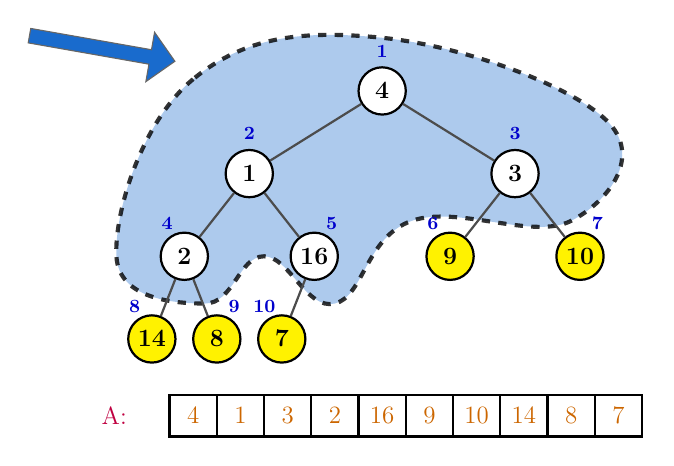
\begin{tikzpicture}[
					scale=0.75, transform shape,
					level distance=1.4cm,
					level 1/.style={sibling distance=4.5cm},
					level 2/.style={sibling distance=2.2cm},
					level 3/.style={sibling distance=1.1cm},
					% Node trong vùng bôi (trắng) - indices 1, 2, 3, 4, 5
					inode/.style={
						circle, draw=black, thick, fill=white, 
						minimum size=0.8cm, inner sep=0pt, font=\bfseries\large
					},
					% Node ngoài vùng bôi (vàng) - indices 6, 7, 8, 9, 10
					lnode/.style={
						circle, draw=black, thick, fill=yellow, 
						minimum size=0.8cm, inner sep=0pt, font=\bfseries\large
					},
					% Chỉ số index (màu xanh dương đậm)
					idx/.style={
						font=\bfseries\small\color{blue!80!black}, above=1pt
					},
					edge from parent/.style={draw=black!70, thick}
					]
					
				% --- VÙNG BAO (BLOB) ĐÃ CHỈNH SỬA ---
				\begin{pgfonlayer}{background}
					\filldraw[draw=black, dashed, line width=1.5pt, fill=codeblue!40, opacity=0.8] 
					plot [smooth cycle, tension=0.7] coordinates {
						(0, 0.9)       % 1. Đỉnh (trên node 4)
						(-3.2, 0.2)    % 2. Bo trái trên
						(-4.5, -2.8)   % 3. Góc trái dưới (bao node 2)
						(-3.0, -3.6)   % 4. Lượn dưới đáy node 2
						(-2.0, -2.8)   % 5. LÕM LÊN (giữa node 2 và 16)
						(-0.8, -3.6)   % 6. Lượn dưới đáy node 16
						(0.5, -2.2)    % 7. CẮT LÊN CAO (để né node 9 màu vàng)
						(3.2, -2.2)    % 8. Lượn dưới node 3
						(3.8, -0.5)    % 9. Bo phải node 3
					};
				\end{pgfonlayer}
					
					% --- 2. CÂY HEAP ---
					% Root: Index 1, Val 4 (White)
					\node[inode, label={[idx]90:1}] (n1) {4}
					child { 
						% Left Child: Index 2, Val 1 (White)
						node[inode, label={[idx]90:2}] (n2) {1}
						child { 
							% LL Child: Index 4, Val 2 (White)
							node[inode, label={[idx]135:4}] (n4) {2} 
							child { node[lnode, label={[idx]135:8}] (n8) {14} } % Yellow
							child { node[lnode, label={[idx]45:9}] (n9) {8} }   % Yellow
						}
						child { 
							% LR Child: Index 5, Val 16 (White)
							node[inode, label={[idx]45:5}] (n5) {16}
							child { node[lnode, label={[idx]135:10}] (n10) {7} } % Yellow
							child[missing]
						}
					}
					child { 
						% Right Child: Index 3, Val 3 (White)
						node[inode, label={[idx]90:3}] (n3) {3}
						child { node[lnode, label={[idx]135:6}] (n6) {9} }  % Yellow
						child { node[lnode, label={[idx]45:7}] (n7) {10} } % Yellow
					};
					
					% --- 3. MŨI TÊN KHỐI ---
					\node[
					single arrow, 
					draw=black!60, 
					fill=codeblue!90, 
					minimum height=2.5cm, 
					single arrow head extend=0.3cm,
					rotate=-10, 
					anchor=tip
					] at (-3.5, 0.5) {};
					
					% --- 4. MẢNG A ---
					\node[anchor=east, font=\large\color{purple}] at (-4.2, -5.5) {A:};
					
					% Vẽ mảng
					\foreach \val [count=\i] in {4, 1, 3, 2, 16, 9, 10, 14, 8, 7} {
						% Tô màu chữ: Index 1-5 màu cam (như hình), 6-10 màu cam
						\node[draw=black, thick, minimum width=0.8cm, minimum height=0.7cm,
						font=\large\color{orange!80!black}, anchor=center] 
						at (-4.0 + \i*0.8, -5.5) {\val};
					}
				\end{tikzpicture}
			\end{column}
		\end{columns}
	\end{frame}
	
	% ==================================================================
	% SLIDE 63: VÍ DỤ 3 - BUILD HEAP 
	% ==================================================================
	\begin{frame}[t]{1. CẤU TRÚC DỮ LIỆU ĐỐNG}
		\textbf{\large \ \ $\gg$ \ Ví dụ 3}
		\begin{flushright}
			\vspace{-0.6cm}
			\begin{center}
				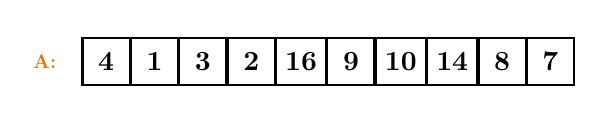
\begin{tikzpicture}[scale=0.6, transform shape]
				
					\matrix[
					matrix of nodes,
					nodes={draw, thick, minimum size=0.6cm, anchor=center, font=\bfseries},
					column sep=-\pgflinewidth,
					row sep=-\pgflinewidth,
					nodes in empty cells,
					ampersand replacement=\&
					] (arr) {
						4 \& 1 \& 3 \& 2 \& 16 \& 9 \& 10 \& 14 \& 8 \& 7 \\
					};
				
					\node[font=\large\bfseries\color{orange!90!black}, anchor=east, xshift=-0.2cm] 
					at (arr.west) {A:};
				\end{tikzpicture}
			\end{center}
		\end{flushright}
		
		\vspace{-0.5cm}
		
		\begin{center}
			\begin{adjustbox}{width=0.88\textwidth}
				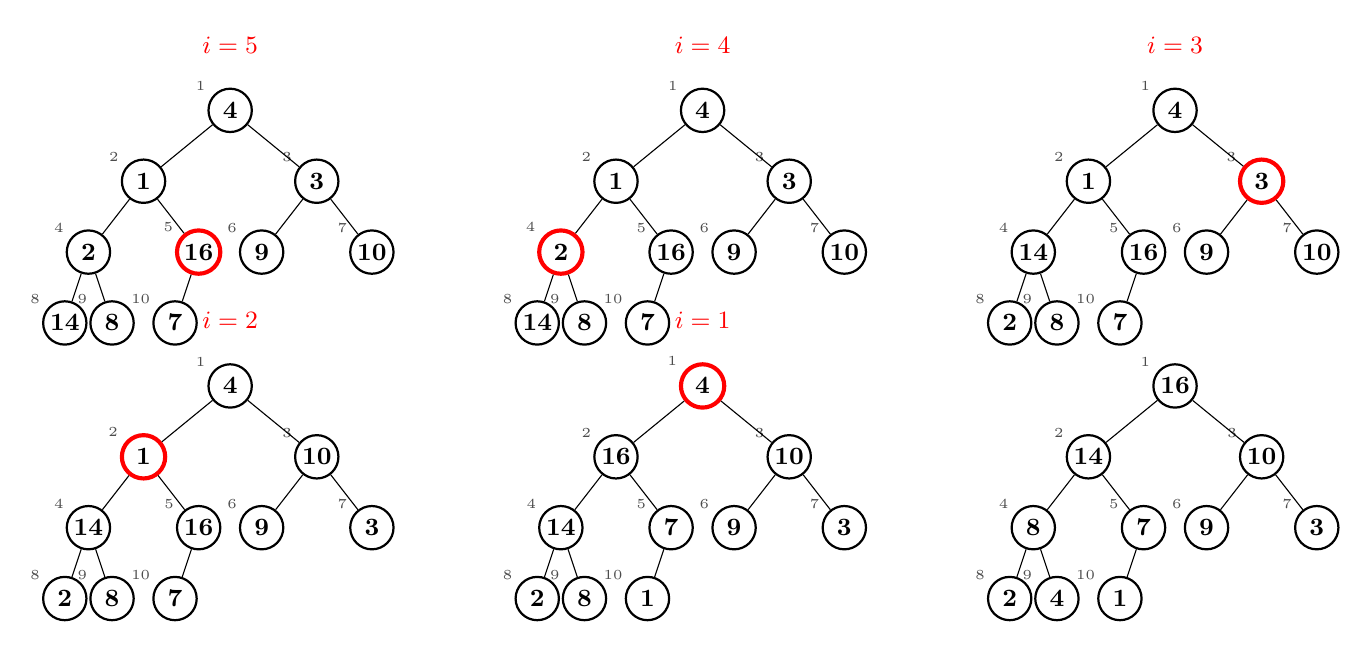
\begin{tikzpicture}[
					level distance=0.9cm,
					level 1/.style={sibling distance=2.2cm},
					level 2/.style={sibling distance=1.4cm},
					level 3/.style={sibling distance=0.6cm},
					norm/.style={
						circle, draw=black, thick, 
						inner sep=0pt, minimum size=0.55cm, 
						font=\bfseries\small
					},
					hi/.style={
						circle, draw=red, line width=1.5pt, 
						text=black, inner sep=0pt, minimum size=0.55cm, 
						font=\bfseries\small
					},
					idx/.style={
						font=\tiny, color=black!70, anchor=south east, inner sep=1pt, xshift=-2pt
					},
					title_label/.style={
						font=\small\bfseries\color{red}, anchor=south, yshift=0.1cm
					}
					]
					
					
					% --- TREE 1 (i=5) ---
					\begin{scope}[xshift=-6cm, yshift=0cm]
						\node[title_label] at (0,0.5) {$i=5$};
						\node[norm, label={[idx]135:1}] (n1) {4}
						child { node[norm, label={[idx]135:2}] {1} 
							child { node[norm, label={[idx]135:4}] {2} 
								child { node[norm, label={[idx]135:8}] {14} }
								child { node[norm, label={[idx]135:9}] {8} }
							}
							child { node[hi, label={[idx]135:5}] {16} 
								child { node[norm, label={[idx]135:10}] {7} }
								child[missing]
							}
						}
						child { node[norm, label={[idx]135:3}] {3} 
							child { node[norm, label={[idx]135:6}] {9} }
							child { node[norm, label={[idx]135:7}] {10} }
						};
					\end{scope}
					
					% --- TREE 2 (i=4) ---
					\begin{scope}[xshift=0cm, yshift=0cm]
						\node[title_label] at (0,0.5) {$i=4$};
						\node[norm, label={[idx]135:1}] {4}
						child { node[norm, label={[idx]135:2}] {1} 
							child { node[hi, label={[idx]135:4}] {2} 
								child { node[norm, label={[idx]135:8}] {14} }
								child { node[norm, label={[idx]135:9}] {8} }
							}
							child { node[norm, label={[idx]135:5}] {16} 
								child { node[norm, label={[idx]135:10}] {7} }
								child[missing]
							}
						}
						child { node[norm, label={[idx]135:3}] {3} 
							child { node[norm, label={[idx]135:6}] {9} }
							child { node[norm, label={[idx]135:7}] {10} }
						};
					\end{scope}
					
					% --- TREE 3 (i=3) ---
					\begin{scope}[xshift=6cm, yshift=0cm]
						\node[title_label] at (0,0.5) {$i=3$};
						\node[norm, label={[idx]135:1}] {4}
						child { node[norm, label={[idx]135:2}] {1} 
							child { node[norm, label={[idx]135:4}] {14} 
								child { node[norm, label={[idx]135:8}] {2} }
								child { node[norm, label={[idx]135:9}] {8} }
							}
							child { node[norm, label={[idx]135:5}] {16} 
								child { node[norm, label={[idx]135:10}] {7} }
								child[missing]
							}
						}
						child { node[hi, label={[idx]135:3}] {3} 
							child { node[norm, label={[idx]135:6}] {9} }
							child { node[norm, label={[idx]135:7}] {10} }
						};
					\end{scope}
					
					% --- TREE 4 (i=2) ---
					\begin{scope}[xshift=-6cm, yshift=-3.5cm]
						\node[title_label] at (0,0.5) {$i=2$};
						\node[norm, label={[idx]135:1}] {4}
						child { node[hi, label={[idx]135:2}] {1} 
							child { node[norm, label={[idx]135:4}] {14} 
								child { node[norm, label={[idx]135:8}] {2} }
								child { node[norm, label={[idx]135:9}] {8} }
							}
							child { node[norm, label={[idx]135:5}] {16} 
								child { node[norm, label={[idx]135:10}] {7} }
								child[missing]
							}
						}
						child { node[norm, label={[idx]135:3}] {10} 
							child { node[norm, label={[idx]135:6}] {9} }
							child { node[norm, label={[idx]135:7}] {3} }
						};
					\end{scope}
					
					% --- TREE 5 (i=1) ---
					\begin{scope}[xshift=0cm, yshift=-3.5cm]
						\node[title_label] at (0,0.5) {$i=1$};
						\node[hi, label={[idx]135:1}] {4} 
						child { node[norm, label={[idx]135:2}] {16} 
							child { node[norm, label={[idx]135:4}] {14} 
								child { node[norm, label={[idx]135:8}] {2} }
								child { node[norm, label={[idx]135:9}] {8} }
							}
							child { node[norm, label={[idx]135:5}] {7} 
								child { node[norm, label={[idx]135:10}] {1} }
								child[missing]
							}
						}
						child { node[norm, label={[idx]135:3}] {10} 
							child { node[norm, label={[idx]135:6}] {9} }
							child { node[norm, label={[idx]135:7}] {3} }
						};
					\end{scope}
					
					% --- TREE 6 (Kết quả) ---
					\begin{scope}[xshift=6cm, yshift=-3.5cm]
						\node[norm, label={[idx]135:1}] {16}
						child { node[norm, label={[idx]135:2}] {14} 
							child { node[norm, label={[idx]135:4}] {8} 
								child { node[norm, label={[idx]135:8}] {2} }
								child { node[norm, label={[idx]135:9}] {4} }
							}
							child { node[norm, label={[idx]135:5}] {7} 
								child { node[norm, label={[idx]135:10}] {1} }
								child[missing]
							}
						}
						child { node[norm, label={[idx]135:3}] {10} 
							child { node[norm, label={[idx]135:6}] {9} }
							child { node[norm, label={[idx]135:7}] {3} }
						};
					\end{scope}
					
				\end{tikzpicture}
			\end{adjustbox}
		\end{center}
	\end{frame}
	
		% ==================================================================
		% SLIDE 64: THỜI GIAN TÍNH CỦA BUILD-MAX-HEAP
		% ==================================================================
		\begin{frame}[t]{1. CẤU TRÚC DỮ LIỆU ĐỐNG}
			\setlength{\leftmargini}{-1.2em}
			\small
			\vspace{-0.1cm}
			\textbf{\large $\gg$ Thời gian tính của Build-Max-Heap}
			
			\begin{itemize}
				\item Heapify đòi hỏi thời gian $O(h) \Rightarrow$ chi phí của Heapify ở nút $i$ là tỷ lệ với chiều cao của nút $i$ trên cây $\Rightarrow T(n) = \sum_{i=0}^{h} n_i h_i = \sum_{i=0}^{h} 2^i (h-i) = O(n)$
			\end{itemize}
			
			\vspace{-0.3cm}
			
			\begin{center}
				\begin{adjustbox}{width=0.98\textwidth}
					\begin{tikzpicture}[
						level distance=1.3cm,
						level 1/.style={sibling distance=5.5cm},
						level 2/.style={sibling distance=2.8cm},
						level 3/.style={sibling distance=1.4cm},
						every node/.style={font=\sffamily\large},
						tree_node/.style={
							circle, draw=black, thick, 
							minimum size=0.6cm, inner sep=0pt
						},
						red_arrow/.style={
							<->, >=Stealth,  
							red!90!black, line width=2pt, 
							bend right=10    % Độ cong vừa phải để băng qua cây
						},
						header_line/.style={
							draw, black, ultra thick, shorten >= -5pt, shorten <= -5pt
						}
						]
						% --- 1. VẼ CÂY (Giữ nguyên) ---
						\node[tree_node] (root) {}
						child { node[tree_node] (L1_L) {} 
							child { node[tree_node] (L2_LL) {} 
								child { node[tree_node] (L3_LLL) {} }
								child { node[tree_node] (L3_LLR) {} }
							}
							child { node[tree_node] (L2_LR) {} 
								child { node[tree_node] (L3_LRL) {} }
								child { node[tree_node] (L3_LRR) {} }
							}
						}
						child { node[tree_node] (L1_R) {} 
							child { node[tree_node] (L2_RL) {} 
								child { node[tree_node] (L3_RLL) {} }
								child { node[tree_node] (L3_RLR) {} }
							}
							child { node[tree_node] (L2_RR) {} 
								child { node[tree_node] (L3_RRL) {} }
								child { node[tree_node] (L3_RRR) {} }
							}
						};
						
						% --- 2. NHÃN BÊN TRÁI (Chiều cao) ---
						\node[anchor=east] (H0) at (-6.5, 0) {$h_0 = 3 \ (\lfloor \log n \rfloor)$};
						\node[anchor=east] (H1) at (-6.5, -1.3) {$h_1 = 2$};
						\node[anchor=east] (H2) at (-6.5, -2.6) {$h_2 = 1$};
						\node[anchor=east] (H3) at (-6.5, -3.9) {$h_3 = 0$};
						
						\node[anchor=south west, font=\bfseries] (H_Left) at (-8.5, 0.4) {Chiều cao};
						\draw[header_line] (H_Left.south west) -- (H_Left.south east);
						
						% --- 3. NHÃN BÊN PHẢI (Mức & Số lượng nút) ---
						% Cột Mức (i) - Giữ nguyên vị trí để tham chiếu visual
						\node[anchor=west] (I0) at (5.5, 0) {$i=0$};
						\node[anchor=west] (I1) at (5.5, -1.3) {$i=1$};
						\node[anchor=west] (I2) at (5.5, -2.6) {$i=2$};
						\node[anchor=west] (I3) at (5.5, -3.9) {$i=3 \ (\lfloor \log n \rfloor)$};
						
						% Cột Số lượng (2^i) - Đích đến của mũi tên
						\node[anchor=west] (N0) at (8.5, 0) {$2^0$};
						\node[anchor=west] (N1) at (8.5, -1.3) {$2^1$};
						\node[anchor=west] (N2) at (8.5, -2.6) {$2^2$};
						\node[anchor=west] (N3) at (8.5, -3.9) {$2^3$};
						
						% Header Phải
						\node[anchor=south west, font=\bfseries] (H_Mid) at (5.5, 0.4) {Mức};
						\draw[header_line] (H_Mid.south west) -- (H_Mid.south east);
						
						\node[anchor=south west, font=\bfseries] (H_Right) at (8.5, 0.4) {Số lượng nút};
						\draw[header_line] (H_Right.south west) -- (H_Right.south east);
						
						% --- 4. MŨI TÊN ĐỎ (ĐÃ SỬA) ---
						% Vẽ mũi tên 2 chiều từ H (Trái) sang N (Phải - Số lượng nút)
						\draw[red_arrow] (H0.east) to (N0.west);
						\draw[red_arrow] (H1.east) to (N1.west);
						\draw[red_arrow] (H2.east) to (N2.west);
						\draw[red_arrow] (H3.east) to (N3.west);
						
						% --- 5. CHÚ THÍCH DƯỚI CÙNG ---
						\node[anchor=west, blue!80!black, font=\large] at (-6.5, -5.2) 
						{$h_i = h - i \quad$ chiều cao của đống gốc tại mức $i$};
						\node[anchor=west, blue!80!black, font=\large] at (-6.5, -6.0) 
						{$n_i = 2^i \quad \quad \ $ số lượng nút ở mức $i$};
						
					\end{tikzpicture}
				\end{adjustbox}
			\end{center}
		\end{frame}
		
		\subsection{Sắp xếp vun đống}
		
		% =========================
		% SLIDE 66: 2. SẮP XẾP VUN ĐỐNG (Sơ đồ của thuật toán)
		% =========================
		\begin{frame}[t]{2. SẮP XẾP VUN ĐỐNG}
			\setlength{\leftmargini}{-1.2em}
			\small
			
			{\large\textbf{Sơ đồ của thuật toán:}}
			
			\vspace{0.2cm}
			
			\begin{itemize}
				\item Tạo đống max-heap từ mảng đã cho
				\item Đổi chỗ gốc (phần tử lớn nhất) với phần tử cuối cùng trong mảng
				\item Loại bỏ nút cuối cùng bằng cách giảm kích thước của đống đi $1$
				\item Thực hiện Max-Heapify đối với gốc mới
				\item Lặp lại quá trình cho đến khi đống chỉ còn $1$ nút
			\end{itemize}
			
		\end{frame}
		
		% ==================================================================
		% SLIDE: VÍ DỤ 4 - HEAP SORT (ĐÃ SỬA MŨI TÊN ĐẸP HƠN)
		% ==================================================================
		\begin{frame}[t]{2. SẮP XẾP VUN ĐỐNG}
			\setlength{\leftmargini}{-1.2em}
			\small
			
			\begin{itemize}
				\item Ví dụ 4 \large $A=[7, 4, 3, 1, 2]$
			\end{itemize}
			
			\vspace{-0.4cm}
			
			\begin{center}
				\resizebox{0.8\textwidth}{!}{ % Co giãn vừa khít slide
					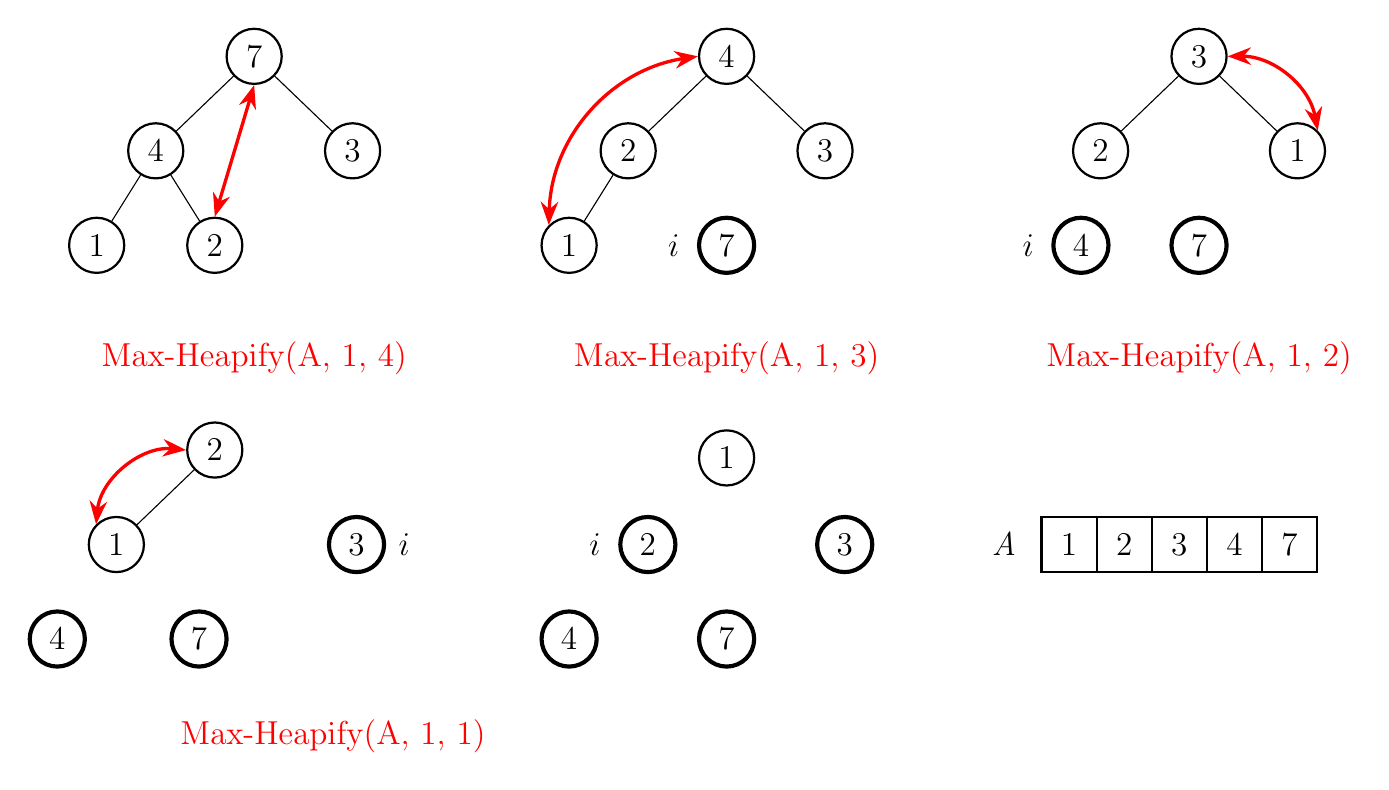
\begin{tikzpicture}[
						level distance=1.2cm,
						level 1/.style={sibling distance=2.5cm},
						level 2/.style={sibling distance=1.5cm},
						% Node thường
						norm/.style={
							circle, draw=black, thick, 
							minimum size=0.7cm, inner sep=0pt, 
							font=\large
						},
						% Node đã sắp xếp (vòng tròn đậm hơn)
						sorted/.style={
							circle, draw=black, line width=1.5pt, 
							minimum size=0.7cm, inner sep=0pt, 
							font=\large
						},
						% Mũi tên đỏ swap (2 đầu)
						swap_arrow/.style={
							<->, >=Stealth, red, line width=1.2pt
						},
						% Nhãn caption màu đỏ
						caption_red/.style={
							font=\large\color{red}, anchor=north, yshift=-0.5cm
						},
						% Nhãn i
						label_i/.style={
							font=\large\itshape, anchor=east, xshift=-0.1cm
						}
						]
						
						% --- BƯỚC 1: Max-Heapify(A, 1, 4) ---
						\begin{scope}[shift={(0,0)}]
							% Cây: 7 -> (4, 3), 4 -> (1, 2)
							\node[norm] (r) at (0,0) {7}
							child { node[norm] (n4) {4} 
								child { node[norm] (n1) {1} }
								child { node[norm] (n2) {2} }
							}
							child { node[norm] (n3) {3} };
							
							% Mũi tên thẳng nối 7 và 2 (như hình mẫu)
							\draw[swap_arrow] (n2.north) -- (r.south);
							
							\node[caption_red] at (0,-3) {Max-Heapify(A, 1, 4)};
						\end{scope}
						
						% --- BƯỚC 2: Max-Heapify(A, 1, 3) ---
						\begin{scope}[shift={(6,0)}]
							% Cây: 4 -> (2, 3), 2 -> (1)
							\node[norm] (r) at (0,0) {4}
							child { node[norm] (n2) {2} 
								child { node[norm] (n1) {1} }
								child[missing]
							}
							child { node[norm] (n3) {3} };
							
							% Node 7 (sorted)
							\node[sorted] (n7) at (0,-2.4) {7};
							\node[label_i] at (n7.west) {$i$};
							
							% Mũi tên cong nhẹ sang trái
							\draw[swap_arrow, bend left=40] (n1.north west) to (r.west);
							
							\node[caption_red] at (0,-3) {Max-Heapify(A, 1, 3)};
						\end{scope}
						
						% --- BƯỚC 3: Max-Heapify(A, 1, 2) ---
						\begin{scope}[shift={(12,0)}]
							% Cây: 3 -> (2, 1)
							\node[norm] (r) at (0,0) {3}
							child { node[norm] (n2) {2} }
							child { node[norm] (n1) {1} };
							
							% Node 4, 7 (sorted)
							\node[sorted] (n4) at (-1.5,-2.4) {4};
							\node[label_i] at (n4.west) {$i$};
							\node[sorted] (n7) at (0,-2.4) {7};
							
							% Mũi tên cong nhẹ sang phải
							\draw[swap_arrow, bend right=40] (n1.north east) to (r.east);
							
							\node[caption_red] at (0,-3) {Max-Heapify(A, 1, 2)};
						\end{scope}
						
						% --- HÀNG 2 ---
						
						% --- BƯỚC 4: Max-Heapify(A, 1, 1) ---
						\begin{scope}[shift={(-0.5,-5.0)}]
							% Cây: 2 -> (1)
							\node[norm] (r) at (0,0) {2}
							child { node[norm] (n1) {1} }
							child[missing];
							
							% Node sorted: 3, 4, 7
							\node[sorted] (n3) at (1.8,-1.2) {3}; % Node 3 nằm ngang hàng i
							\node[label_i] at (2.7,-1.2) {$i$}; 
							
							\node[sorted] (n4) at (-2,-2.4) {4};
							\node[sorted] (n7) at (-0.2,-2.4) {7};
							
							% Mũi tên cong nhẹ sang trái
							\draw[swap_arrow, bend left=45] (n1.north west) to (r.west);
							
							\node[caption_red] at (1.5,-2.8) {Max-Heapify(A, 1, 1)};
						\end{scope}
						
						% --- BƯỚC 5: Kết quả ---
						\begin{scope}[shift={(6,-5.0)}]
							% Cây: 1 (gốc)
							\node[norm] (n1) at (0, -0.1) {1}; % Node 1 đứng riêng ở trên
							\node[label] at (n1.west) {}; % Placeholder
							
							% Node sorted: 2, 3, 4, 7
							\node[sorted] (n2) at (-1,-1.2) {2};
							\node[label_i] at (n2.west) {$i$};
							
							\node[sorted] (n3) at (1.5,-1.2) {3};
							\node[sorted] (n4) at (-2,-2.4) {4};
							\node[sorted] (n7) at (0,-2.4) {7};
							
							% Vẽ mảng kết quả A
							\begin{scope}[shift={(4,-1.2)}]
								\node[font=\large\itshape, anchor=east] at (-0.2, 0) {A};
								\foreach \val [count=\i] in {1, 2, 3, 4, 7} {
									\node[draw, thick, minimum width=0.7cm, minimum height=0.7cm, font=\large] 
									at (\i*0.7 - 0.35, 0) {\val};
								}
							\end{scope}
						\end{scope}
						
					\end{tikzpicture}
				}
			\end{center}
		\end{frame}
		
		% =========================
		% SLIDE 68: 2. SẮP XẾP VUN ĐỐNG (HeapSort(A))
		% =========================
		\begin{frame}[t,fragile]{2. SẮP XẾP VUN ĐỐNG}
			\setlength{\leftmargini}{-1.2em}
			\small
			
			\begin{itemize}
				\item \textit{Algorithm:} \large \textbf{HeapSort(A)}
			\end{itemize}
			
			\vspace{0.15cm}
			
			\begin{center}
				\begin{tcolorbox}[
					width=0.78\textwidth,
					colback=white,
					colframe=white,
					boxrule=0pt,
					arc=0pt,
					left=0pt,right=0pt,top=0pt,bottom=0pt
					]
					\begin{enumerate}
						\item Build-Max-Heap(A)
						\item \textbf{for} $i \leftarrow \text{length}[A]$ \textbf{downto} $2$
						\item \hspace{1.15em} \textbf{do} exchange $A[1] \leftrightarrow A[i]$
						\item \hspace{1.15em} Max-Heapify(A, 1, $i-1$)
					\end{enumerate}
				\end{tcolorbox}
			\end{center}
			
			\vspace{0.35cm}
			
			\begin{itemize}
				\item Thời gian tính: $O(n\log n)$
			\end{itemize}
			
		\end{frame}
		
	
		{\HUSTUseBackground{theme_hust_oneside.pdf}
		\begin{frame}
			\ifdefstring{\insertaspectratio}{169}{
				\placecontent{0.355\paperwidth}{0.410\paperheight}{0.640\paperwidth}{
					\color{HUSTRed}\bfseries\fontsize{28pt}{36pt}\selectfont\centering
					THANK YOU!
				}
			}{}
			\ifdefstring{\insertaspectratio}{43}{
				\placecontent{0.355\paperwidth}{0.440\paperheight}{0.640\paperwidth}{
					\color{HUSTRed}\bfseries\fontsize{28pt}{36pt}\selectfont\centering
					THANK YOU!
				}
			}{}
		\end{frame}
	}
	


	
\end{document} 